%%% LaTeX-Vorlage Version 1.8 %%%

% Grundlegende Dokumenteneigenschaften gemäß DHBW-Vorgaben
\documentclass[a4paper,fontsize=11pt,oneside,parskip=half,headings=normal]{scrreprt} 
% \usepackage{showframe} % nur für Kontrolle der Ränder 

%%% Präambel einbinden (mit Festlegungen gemäß DHBW-Vorgaben) %%%
%%% Präambel %%%
% hier sollten keine Änderungen erforderlich sein
%
\usepackage[utf8]{inputenc}   % Zeichencodierung UTF-8 für Eingabe-Dateien
\usepackage[T1]{fontenc}      % Darstellung von Umlauten im PDF

\usepackage{listings}         % für Einbindung von Code-Listings
\lstset{numbers=left,numberstyle=\tiny,numbersep=5pt,texcl=true}
\lstset{literate=             % erlaubt Sonderzeichen in Code-Listings 
{Ö}{{\"O}}1
{Ä}{{\"A}}1
{Ü}{{\"U}}1
{ß}{{\ss}}2
{ü}{{\"u}}1
{ä}{{\"a}}1
{ö}{{\"o}}1
{€}{{\euro}}1
}

\usepackage[
  inner=35mm,outer=15mm,top=25mm,
  bottom=20mm,foot=12mm,includefoot
]{geometry}                 % Einstellungen für Ränder

\usepackage[ngerman]{babel} % Spracheinstellungen Deutsch
\usepackage[babel,german=quotes]{csquotes} % deutsche Anf.zeichen
\usepackage{enumerate}      % anpassbare Nummerier./Aufz.
\usepackage{graphicx}       % Einbinden von Grafiken
\usepackage[onehalfspacing]{setspace} % anderthalbzeilig

\usepackage{blindtext}      % Textgenerierung für Testzwecke
\usepackage{color}          % Verwendung von Farbe 

\usepackage{acronym}        % für ein Abkürzungsverzeichnis

\usepackage[                % Biblatex
  backend=biber,
  bibstyle=_dhbw_authoryear,maxbibnames=99,
  citestyle=authoryear,     
  uniquename=true, useprefix=true,
  bibencoding=utf8]{biblatex}
%kein Punkt am Ende bei \footcite
%http://www.golatex.de/footcite-ohne-punkt-am-schluss-t4865.html
\renewcommand{\bibfootnotewrapper}[1]{\bibsentence#1}


%Reihenfolge der Autorennamen
%   
% http://golatex.de/viewtopic,p,80448.html#80448
% Argumente: siehe http://texwelt.de/blog/modifizieren-eines-biblatex-stils/
\DeclareNameFormat{sortname}{% Bibliographie
  \ifnum\value{uniquename}=0 % Normalfall
    \ifuseprefix%
      {%
         \usebibmacro{name:family-given}
           {\namepartfamily}
           {\namepartgiveni}
           {\namepartprefix}
           {\namepartsuffixi}%
       }
      {%
         \usebibmacro{name:family-given}
           {\namepartfamily}
           {\namepartgiveni}
           {\namepartprefixi}
           {\namepartsuffixi}%
       }%
  \fi
  \ifnum\value{uniquename}=1% falls nicht eindeutig, abgek. Vorname 
      {%
         \usebibmacro{name:family-given}
           {\namepartfamily}
           {\namepartgiveni}
           {\namepartprefix}
           {\namepartsuffix}%
       }%
  \fi
  \ifnum\value{uniquename}=2% falls nicht eindeutig, ganzer Vorname 
      {%
         \usebibmacro{name:family-given}
           {\namepartfamily}
           {\namepartgiven}
           {\namepartprefix}
           {\namepartsuffix}%
       }%
  \fi   
  \usebibmacro{name:andothers}}

\DeclareNameFormat{labelname}{% für Zitate
  \ifnum\value{uniquename}=0 % Normalfall
    \ifuseprefix%
      {%
         \usebibmacro{name:family-given}
           {\namepartfamily}
           {\empty}
           {\namepartprefix}
           {\namepartsuffixi}%
       }
      {%
         \usebibmacro{name:family-given}
           {\namepartfamily}
           {\empty}
           {\namepartprefixi}
           {\namepartsuffixi}%
       }%
  \fi
  \ifnum\value{uniquename}=1% falls nicht eindeutig, abgek. Vorname 
      {%
         \usebibmacro{name:family-given}
           {\namepartfamily}
           {\namepartgiveni}
           {\namepartprefix}
           {\namepartsuffix}%
       }%
  \fi
  \ifnum\value{uniquename}=2% falls nicht eindeutig, ganzer Vorname 
      {%
         \usebibmacro{name:family-given}
           {\namepartfamily}
           {\namepartgiven}
           {\namepartprefix}
           {\namepartsuffix}%
       }%
  \fi   
  \usebibmacro{name:andothers}}
      
  
\DeclareFieldFormat{extrayear}{% = the 'a' in 'Jones 1995a'
  \iffieldnums{labelyear}
    {\mknumalph{#1}}
    {\mknumalph{#1}}}        

\renewcommand*{\multinamedelim}{\addslash}
\renewcommand*{\finalnamedelim}{\addslash}
\renewcommand*{\multilistdelim}{\addslash}
\renewcommand*{\finallistdelim}{\addslash}

\renewcommand{\nameyeardelim}{~}

% Literaturverzeichnis: Doppelpunkt zwischen Name (Jahr): Rest 
% http://de.comp.text.tex.narkive.com/Tn1HUIXB/biblatex-authoryear-und-doppelpunkt
\renewcommand{\labelnamepunct}{\addcolon\addspace}

% damit die Darstellung für Vollzitate von Primärquellen in 
% Fußnoten später auf "nicht fett" geändert werden kann 
% (nur für Zitate von Sekundärliteratur relevant)
\newcommand{\textfett}[1]{\textbf{#1}}

% für Zitate von Sekundärliteratur:
\newcommand{\footcitePrimaerSekundaer}[4]{%
  \renewcommand{\textfett}[1]{##1}%
  \footnote{\fullcite[#2]{#1}, zitiert nach \cite[#4]{#3}}%  
  \renewcommand{\textfett}[1]{\textbf{##1}}%
}

% Im Literaturverzeichnis: Autor (Jahr) fett
\renewbibmacro*{author}{%
  \ifboolexpr{%
    test \ifuseauthor%
    and
    not test {\ifnameundef{author}}
  }
    {\usebibmacro{bbx:dashcheck}
       {\bibnamedash}
       {\usebibmacro{bbx:savehash}%
        \textfett{\printnames{author}}%
        \iffieldundef{authortype}
          {\setunit{\addspace}}
          {\setunit{\addcomma\space}}}%
     \iffieldundef{authortype}
       {}
       {\usebibmacro{authorstrg}%
        \setunit{\addspace}}}%
    {\global\undef\bbx@lasthash
     \usebibmacro{labeltitle}%
     \setunit*{\addspace}}%
  \textfett{\usebibmacro{date+extrayear}}}

% Sonderfall: Quelle ohne Autor, aber mit Herausgeber
% Name des Herausgebers wird fett gedruckt
\renewbibmacro*{bbx:editor}[1]{%
  \ifboolexpr{%
    test \ifuseeditor%
    and
    not test {\ifnameundef{editor}}
  }
    {\usebibmacro{bbx:dashcheck}
       {\bibnamedash}
       {\textfett{\printnames{editor}}%
        \setunit{\addcomma\space}%
        \usebibmacro{bbx:savehash}}%
     \usebibmacro{#1}%
     \clearname{editor}%
     \setunit{\addspace}}%
    {\global\undef\bbx@lasthash
     \usebibmacro{labeltitle}%
     \setunit*{\addspace}}%
  \textfett{\usebibmacro{date+extrayear}}}

% Anpassungen für deutsche Sprache
\DefineBibliographyStrings{ngerman}{%
	nodate = {{o.J.}},
	urlseen = {{Abruf:}},
	ibidem = {{ebenda}}
}

% keine Anführungszeichen beim Titel im Literaturverzeichnis
\DeclareFieldFormat[article,book,inbook,inproceedings,manual,misc,phdthesis,thesis,online,report]{title}{#1\isdot}

\newcommand{\literaturverzeichnis}{%
% nur Literaturverzeichnis
% (als eigenes Kapitel)
\phantomsection
\addcontentsline{toc}{chapter}{Literaturverzeichnis}
\spezialkopfzeile{Literaturverzeichnis}
\defbibheading{lit}{\chapter*{Literaturverzeichnis}}
\label{chapter:quellen}
\printbibliography[heading=lit,notkeyword=ausblenden]
} % mit DHBW-spezifischen Einstellungen

\usepackage{hyperref}       % URL-Formatierung, klickbare Verweise

\usepackage{tocloft}        % für Verzeichnis der Anhänge

\newcounter{anhcnt}
\setcounter{anhcnt}{0}
\newlistof{anhang}{app}{}

\newcommand{\anhang}[1]{%
  \refstepcounter{anhcnt}
  \setcounter{anhteilcnt}{0}
  \section*{Anhang \theanhcnt: #1}
  \addcontentsline{app}{section}{\protect\numberline{Anhang \theanhcnt}#1}\par
}

\newcounter{anhteilcnt}
\setcounter{anhteilcnt}{0}

\newcommand{\anhangteil}[1]{%
	\refstepcounter{anhteilcnt}
	\subsection*{Anhang~\arabic{anhcnt}/\arabic{anhteilcnt}: #1}
	\addcontentsline{app}{subsection}{\protect\numberline{Anhang \theanhcnt/\arabic{anhteilcnt}}#1}\par
}

\renewcommand{\theanhteilcnt}{Anhang \theanhcnt/\arabic{anhteilcnt}}

% vgl. S. 4 Paket-Beschreibung tocloft 	
% Einrückungen für Anhangverzeichnis
\makeatletter
\newcommand{\abstaendeanhangverzeichnis}{
\renewcommand*{\l@section}{\@dottedtocline{1}{0em}{5.5em}}
\renewcommand*{\l@subsection}{\@dottedtocline{2}{2.3em}{6.5em}}
}
\makeatother

% Abbildungs- und Tabellenverzeichnis
% Bezeichnungen
\renewcaptionname{ngerman}{\figurename}{Abb.}
\renewcaptionname{ngerman}{\tablename}{Tab.}
% Einrückungen
\makeatletter
\renewcommand*{\l@figure}{\@dottedtocline{1}{0em}{2.3em}}
\renewcommand*{\l@table}{\@dottedtocline{1}{0em}{2.3em}}
\makeatother


\usepackage{chngcntr}                % fortlaufende Zähler für Fußnoten, Abbildungen und Tabellen
\counterwithout{figure}{chapter}
\counterwithout{table}{chapter}
\counterwithout{footnote}{chapter}

\usepackage[automark]{scrlayer-scrpage} 
%% Definitionen für Kopf- und Fußzeile auf normalen Seiten
\defpagestyle{kopfzeile}
{% Kopfdefinition
  (\textwidth,0pt)    % Länge der oberen Linie,Dicke der oberen Linie       
  {} % Definition für linke Seiten im doppelseitigen Layout
  {} % Definition für rechte Seiten im doppelseitigen Layout      
  {  % Definition für Seiten im einseitigen Layout
	\makebox[0pt][l]{\rightmark}% 
	\makebox[\linewidth]{}% 
  }        
  (\textwidth, 0.4pt) % Untere Linienlänge, Untere Liniendicke
}
{% Fußdefinition
  (\textwidth,0pt)    % Obere Linienlänge, Obere Liniendicke
  {} % Definition für linke Seiten im doppelseitigen Layout
  {} % Definition für rechte Seiten im doppelseitigen Layout
  {  % Definition für Seiten im einseitigen Layout
    \makebox[\linewidth]{}%
    \makebox[0pt][r]{\pagemark}%
  }
  (\textwidth, 0pt)   % Länge der unteren Linie,Dicke der unteren Linie
}

%% Definitionen für Kopf- und Fußzeile auf ersten Seiten eines Kapitels
\defpagestyle{kapitelkopfzeile}
{% Kopfdefinition
  (\textwidth,0pt)    % Länge der oberen Linie,Dicke der oberen Linie       
  {} % Definition für linke Seiten im doppelseitigen Layout
  {} % Definition für rechte Seiten im doppelseitigen Layout      
  {}  % Definition für Seiten im einseitigen Layout
  (\textwidth, 0pt) % Untere Linienlänge, Untere Liniendicke
}
{% Fußdefinition
  (\textwidth,0pt)    % Obere Linienlänge, Obere Liniendicke
  {} % Definition für linke Seiten im doppelseitigen Layout
  {} % Definition für rechte Seiten im doppelseitigen Layout
  {  % Definition für Seiten im einseitigen Layout
    \makebox[\linewidth]{}%
    \makebox[0pt][r]{\pagemark}%
  }
  (\textwidth, 0pt)   % Länge der unteren Linie,Dicke der unteren Linie
}

%% Definitionen für Kopf- und Fußzeile im Anhang und bei Quellenverzeichnisse
\newcommand{\spezialkopfzeileBezeichnung}{}
\defpagestyle{spezialkopfzeile}
{% Kopfdefinition
  (\textwidth,0pt)    % Länge der oberen Linie,Dicke der oberen Linie       
  {} % Definition für linke Seiten im doppelseitigen Layout
  {} % Definition für rechte Seiten im doppelseitigen Layout      
  {  % Definition für Seiten im einseitigen Layout
	\makebox[0pt][l]{\spezialkopfzeileBezeichnung}% 
	\makebox[\linewidth]{}% 
  }        
  (\textwidth, 0.4pt) % Untere Linienlänge, Untere Liniendicke
}
{% Fußdefinition
  (\textwidth,0pt)    % Obere Linienlänge, Obere Liniendicke
  {} % Definition für linke Seiten im doppelseitigen Layout
  {} % Definition für rechte Seiten im doppelseitigen Layout
  {  % Definition für Seiten im einseitigen Layout
    \makebox[\linewidth]{}%
    \makebox[0pt][r]{\pagemark}%
  }
  (\textwidth, 0pt)   % Länge der unteren Linie,Dicke der unteren Linie
}
            
\newcommand\spezialkopfzeile[1]{%
  \renewcommand\spezialkopfzeileBezeichnung{#1}
  \pagestyle{spezialkopfzeile}
}
                
% Standard-Pagestyle auswählen
\pagestyle{kopfzeile}

% keine Kopfzeile anzeigen auf Seiten, auf denen ein 
% Kapitel beginnt oder das Inhalts-/Abbildungs-/Tabellenverzeichnis steht 
\renewcommand{\chapterpagestyle}{kapitelkopfzeile}
\tocloftpagestyle{kapitelkopfzeile}

		 % für schöne Kopfzeilen 

\usepackage{textcomp}            % erlaubt EUR-Zeichen in Eingabedatei
\usepackage{eurosym}             % offizielles EUR-Symbol in Ausgabe
\renewcommand{\texteuro}{\euro}  % ACHTUNG: nach hyperref aufrufen!

\usepackage{scrhack}             % stellt Kompatibilität zw. KOMA-Script
                                 % (scrreprt) und anderen Paketen her

\usepackage{float}
                                 
% Anpassung der Abstände bei Kapitelüberschriften
% (betrifft auch Inhalts-, Abbildungs- und Tabellenverzeichnis)
\renewcommand*\chapterheadstartvskip{\vspace*{-\topskip}}
\newcommand{\myBeforeTitleSkip}{1mm}
\newcommand{\myAfterTitleSkip}{10mm}
\setlength\cftbeforetoctitleskip{\myBeforeTitleSkip}
\setlength\cftbeforeloftitleskip{\myBeforeTitleSkip}
\setlength\cftbeforelottitleskip{\myBeforeTitleSkip}

\setlength\cftaftertoctitleskip{\myAfterTitleSkip}
\setlength\cftafterloftitleskip{\myAfterTitleSkip}
\setlength\cftafterlottitleskip{\myAfterTitleSkip}                                                            
%%% Ende der Präambel %%%

%%% Name der eigenen Literatur-Datenbank (ggf. anpassen) %%%
\bibliography{includes/literatur.bib}

\begin{document}
%%% Deckblatt einbinden %%% 
% Anpassungen nötig (Name, Titel etc.)
% HIER EDITIEREN: 
% Typ der Arbeit (für Deckblatt und Metadaten)
% - bitte Zutreffendes auswählen
%\newcommand{\typMeinerArbeit}{1. Projektarbeit} 
%\newcommand{\typMeinerArbeit}{2. Projektarbeit} 
%\newcommand{\typMeinerArbeit}{Seminararbeit} 
\newcommand{\typMeinerArbeit}{Projekt / Integrationsseminar} 

% Thema der Arbeit (für ehrenwörtliche Erklärung, ohne Umbrüche)
% HIER EDITIEREN: 
\newcommand{\themaMeinerArbeit}{Erstellung eines Wissensquiz für die Einführung von RAPLA an der DHBW Stuttgart}

% Vorname, Name der Autorin/des Autors (für Titelseite und Metadaten)
% HIER EDITIEREN:
\newcommand{\meinNameSB}{Simon Burbiel}
\newcommand{\meinNameLG}{Lukas Großerhode}
\newcommand{\meinNameSS}{Simon Spitzer}
\newcommand{\meinNameTK}{Tim Keicher}
\newcommand{\meinNameDS}{David Stark}

\thispagestyle{empty}

\begin{spacing}{1}
\begin{center}	
~\vspace{0mm}

% HIER EDITIEREN: Titel der Arbeit
{\sffamily
\LARGE  
% \Large  % bei sehr langen Titeln ggf. etwas kleinere Schriftart wählen
\textbf{Erstellung eines Wissensquiz für die Einführung von RAPLA an der DHBW Stuttgart}

% \bigskip
% \textbf{ggf. etwas länger}
}


\vspace{15mm}

% Typ wird automatisch eingefügt (oben festlegen)
{\Large \typMeinerArbeit}

\vspace{1cm}

% HIER ggf. EDITIEREN
vorgelegt am \today 

\vspace{15mm}

Fakultät Wirtschaft und Gesundheit
\medskip

Studiengang Wirtschaftsinformatik
\medskip

% HIER EDITIEREN: Kurs eintragen
Kurs WWI2021F 

\vspace{10mm}

von

\vspace{10mm}

% Vorname und Name wird automatisch eingefügt (oben festlegen) 
{\large\textsc{\meinNameSB}}
\medskip

{\large\textsc{\meinNameLG}}
\medskip

{\large\textsc{\meinNameTK}}
\medskip

{\large\textsc{\meinNameSS}}
\medskip

{\large\textsc{\meinNameDS}}
\medskip

\vspace{10mm}
\end{center}

\vfill




\vspace{1cm}
%(etwas Platz für die Unterschrift der Betreuerin/des Betreuers aus der Ausbildungsstätte)
\end{spacing}

% falls ein Vertraulichkeitsvermerk erforderlich ist,
% die Kommentarzeichen in den nachfolgenden Zeilen entfernen:
 
%\begin{center}
%\small
%\textbf{Vertraulichkeitsvermerk}:
%Der Inhalt dieser Arbeit darf weder als Ganzes noch in Auszügen \\
%Personen außerhalb des Prüfungs- und Evaluationsverfahrens zugänglich gemacht werden, sofern keine anders lautende Genehmigung des Dualen Partners vorliegt. 
%\end{center}

% Meta-Daten für PDF-Datei basierend auf obigen Angaben
\hypersetup{pdftitle={\themaMeinerArbeit}}
\hypersetup{pdfauthor={\meinNameLG}}
\hypersetup{pdfsubject={\typMeinerArbeit\ DHBW Stuttgart \the\year}}

%%% Umstellung der Seiten-Nummerierung auf i, ii, iii ... %%%
\pagenumbering{Roman}

%%% Abstract einbinden (optionale Kurzfassung Ihrer Arbeit) %%%
% \begin{abstract}
\thispagestyle{kapitelkopfzeile}
\textbf{\LaTeX-Vorlage für Projekt-, Seminar- und Bachelorarbeiten}

Bei dem vorliegenden Dokument handelt es sich um eine Vorlage, die
für Projekt-, Seminar- und Bachelorarbeiten im Studiengang
Wirtschaftsinformatik der DHBW Stuttgart verwendet werden kann.

Sie setzt die technischen Vorgaben der Zitierrichtlinien\footnote{Sie finden diese unter \enquote{Prüfungsleistungen} im Studierendenportal (\url{https://www.dhbw-stuttgart.de/studierendenportal/wirtschaftsinformatik/pruefungsleistungen/projekt-/bachelorarbeit/}).} des Studiengangs
(Stand: 07/2023) um.

\emph{Hinweise:} Bitte lesen Sie sich die Zitierrichtlinien unbedingt genau durch. Dieses Dokument ersetzt keine Anleitung oder Einführung in \LaTeX,
für die Nutzung sind daher gewisse Vorkenntnisse unerlässlich. Ein Einstieg in 
\LaTeX\ ist aber weniger schwierig, als es vielleicht auf den ersten Blick scheint
und lohnt sich für das Verfassen wissenschaftlicher Arbeiten in jedem Fall.\footnote{%
so auch \url{http://www.spiegel.de/netzwelt/tech/textsatz-keine-angst-vor-latex-a-549509.html}} 
Als Hilfestellung beim Schreiben eines Dokuments habe ich einen zweiseitigen kompakten \LaTeX-Spickzettel erstellt, der über Moodle verfügbar ist.

Ihre Rückmeldungen und Anregungen zu dieser Vorlage nehme ich gerne per E-Mail an die Adresse
\url{tobias.straub@dhbw-stuttgart.de} entgegen.

--- Prof. Dr. Tobias Straub

\vspace{5em}

\begin{center}\small
\begin{tabular}{ccl}
\multicolumn{3}{c}{\textbf{Versionshistorie}}\\
\hline
1.0	& 05.02.2015 & erste Fassung \\
\hline
1.1 & 16.02.2015 & siehe~\ref{anhang:ReleaseNotes11} \\
\hline
1.2 & 20.04.2015 & siehe~\ref{anhang:ReleaseNotes12} \\
\hline
1.3 & 20.02.2016 & siehe~\ref{anhang:ReleaseNotes13} \\
\hline
1.4 & 24.07.2017 & siehe~\ref{anhang:ReleaseNotes14} \\
\hline
1.5 & 07.01.2018 & siehe~\ref{anhang:ReleaseNotes15} \\
\hline
1.6 & 07.04.2018 & siehe~\ref{anhang:ReleaseNotes16} \\
\hline
1.7 & 12.02.2019 & siehe~\ref{anhang:ReleaseNotes17} \\
\hline
1.8 & 10.02.2020 & siehe~\ref{anhang:ReleaseNotes18} \\
\hline
1.9 & 19.07.2023 & siehe~\ref{anhang:ReleaseNotes19} \\
\end{tabular}
\end{center}

\end{abstract}


\cleardoublepage

%%% Inhalts-, Abbildungs-, Tabellenverzeichnisse %%%
% sollen einzeilig gesetzt werden, um Platz zu sparen 
\begin{spacing}{1}
\tableofcontents
\clearpage
\chapter*{Abkürzungsverzeichnis}
\addcontentsline{toc}{chapter}{Abkürzungsverzeichnis}

\begin{acronym}[RAPLA] 
% Argument definiert die Breite der ersten Spalte anhand des längsten vorkommenden Eintrags
\acro{DHBW}{Duale Hochschule Baden-Württemberg}
\acro{DIN}{Deutsches Institut für Normung}
\acro{ERP}{Enterprise-Resource-Planning}
\acro{MVP}{Minimum Viable Product}
\acro{PM}{Personenmonate}
\acro{RACI}{Responsible, Accountable, Consulted, Informed}
\acro{RAPLA}{Raumplanungsassistent}
\end{acronym}

\clearpage
\thispagestyle{kapitelkopfzeile}
\listoffigures
\phantomsection
\addcontentsline{toc}{chapter}{Abbildungsverzeichnis} % Abb.verz. ins Inh.verz. aufnehmen

\clearpage
\listoftables
\phantomsection
\addcontentsline{toc}{chapter}{Tabellenverzeichnis}   % Tab.verz. ins Inh.verz. aufnehmen
\end{spacing}

%%% Umstellung der Seiten-Nummerierung auf 1, 2, 3 ... %%%
\cleardoublepage
\pagenumbering{arabic}

%%% Ihr eigentlicher Inhalt %%%
% Empfehlung: strukturieren Sie Ihren Text in einzelnen Dateien 
% und binden Sie diese hier mit \input{includes/dateiname.tex} ein

\chapter{Einleitung}
\section{Motivation}
Bei der Einführung neuer Systeme in einem unternehmerischen oder universitären
Kontext ist die Schulung der Endbenutzerinnen und -benutzer ein zentraler Erfolgsfaktor.
\section{Problemstellung}
\section{Zielsetzung}
\section{Vorgehensweise}
\section{Aufbau der Arbeit}


% Die Einführung neuer Systeme und Prozesse erfordert
% stets eine umsichtige und durchdachte Herangehensweise. Diese beginnt bereits
% bei der Systemplanung und erstreckt sich über die Entwicklung bis hin zur abschließenden Migration.
% \footcite[Vgl.][S. 882 ff.]{laudonWirtschaftsinformatikEinfuehrung2016}
% Oftmals kommt es hierbei in der praktischen Umsetzung jedoch zu Fehlern, durch welche die geplante Einführung
% des jeweiligen Systems schlussendlich entweder stark verzögert oder sogar gar nicht stattfindet. Als Beispiel
% hierfür lässt sich die Implementierung eines neuen „\ac{ERP}“-Systems anführen. Auf einer Konferenz für \ac{ERP} benennen
% Becker und Winkelmann 2008 die fehlende Schulung von Mitarbeitenden als zentralen Faktor für das Scheitern eines solchen Projektes.
% \footcite[Vgl.][27]{becker10MoglichkeitenERPProjekt2008}
% Für die erfolgreiche Migration auf ein neues System sei es daher unabdingbar, die Endbenutzerinnen und -benutzer hinsichtlich der
% Bedienung und Funktionen zu schulen, um ein Scheitern der neuen Plattform oder Anwendung und damit eine Vergeudung monetärer und zeitlicher Ressourcen zu vermeiden.  
% \footcite[Vgl.][886]{laudonWirtschaftsinformatikEinfuehrung2016}

% Auch in der Fakultät Wirtschaft an der \acs{DHBW} Stuttgart soll im Jahr 2024 ein neues System eingeführt werden.
% Konkret handelt es sich hierbei um den zentralen Raumplanungsassistenten \acs{RAPLA}, welcher Studiengangsleiterinnen
% und -leiter sowie die zugehörigen Sekretariate bei der Buchung von Räumen unterstützen soll. Bislang erfolgt die Buchung von
% Räumen in der Fakultät Wirtschaft über Excel-Tabellen, wodurch ein sehr hoher Abstimmungsaufwand unter den Studiengängen
% hinsichtlich der effizientesten Belegung von Seminarräumen besteht. Diesem Aspekt kommt insbesondere in Anbetracht einer
% allgemeinen Raumknappheit der Hochschule eine hohe Bedeutung zu. Da \acs{RAPLA} jedoch noch nicht an allen Standorten im Einsatz ist,
% fehlt bislang in vielen Studienzentren das Wissen über den Aufbau, die Beschaffenheit sowie die Funktionen der Anwendung.

% Gegenwärtig wird daher ein statisches Schulungsdokument erstellt, durch welches den jeweiligen Studienzentren sowie Angehörigen der \acs{DHBW} Stuttgart
% bei der Einführung des Raumplanungsassistenten relevante Informationen zur Verfügung gestellt werden.
% Um den Teilnehmerinnen und Teilnehmern der Schulung einen möglichst hohen
% Mehrwert und einen intuitiven Einstieg in die Anwendung zu bieten, soll als Eigenleistung im Rahmen der Projektkonzeption ergänzend zu
% der bereits bestehenden Schulungsdokumentation ein Wissensquiz entwickelt werden, welches direkt in Moodle abgebildet sein wird.
% Dieses soll die Nutzerinnen und Nutzer dazu motivieren, sich mit Anwendung aktiv zu beschäftigen und sie zum Lernen und Ausprobieren
% anregen. Den erfolgreichen Abschluss des Kurses bildet eine persönliche Zertifizierung, welche den Teilnehmenden digital
% zur Verfügung gestellt wird. Die Umsetzung in Moodle wird erreicht, indem in einem ersten Schritt eine umfassende Analyse der Gegebenheiten erfolgt, zu denen bspw.
% die Ziel- und Interessengruppen, vor- und nachgelagerte Prozesse sowie das Programm selbst gehören. Zusätzlich werden die gegenwärtigen
% Schulungsunterlagen gesichtet und die Funktionsfähigkeit von \acs{RAPLA} mittels eines Testzugangs untersucht. Darauf aufbauend wird
% in einem zweiten Schritt eine Seite in Moodle erstellt, auf welcher das Wissensquiz abgebildet sein wird. Im dritten
% Schritt erfolgt eine Evaluation des neuen Schulungsprozesses, welcher eine empirische Validierung mit echten Anwenderinnen und
% Anwendern vorausgeht. Anhand dieser Evaluation soll abschließend hervorgehen, ob und inwiefern die Moodle-Zertifizierung vorteilhaft
% für den operativen Einsatz ist und welche Änderungen und Ergänzungen darauf aufbauend für zukünftige Aktualisierungen in Betracht zu ziehen sind.

% ----


% Daher soll im Rahmen der Studienfächer „Projektkonzeption“, „Projekt“ und „Integrationsseminar“ ein Schulungskonzept erstellt
% werden, welches die jeweiligen Studienzentren sowie Angehörigen der DHBW Stuttgart bei der erfolgreichen Einführung von \acs{RAPLA}
% unterstützt. Dies wird erreicht, indem in einem ersten Schritt eine umfassende Analyse der Gegebenheiten erfolgt, zu denen bspw.
% die Ziel- und Interessengruppen, vor- und nachgelagerte Prozesse sowie das Programm selbst gehören. Zusätzlich werden die gegenwärtigen
% Schulungsunterlagen gesichtet und die Funktionsfähigkeit von \acs{RAPLA} mittels eines Testzugangs untersucht. Darauf aufbauend wird
% in einem zweiten Schritt ein vollumfängliches Schulungskonzept inklusive Schulungsunterlagen erstellt, das Auskunft darüber gibt,
% welche Personenkreise zu welchem Zeitpunkt mit welchen Mitteln zu schulen sind, um das jeweilige Ziel zu erreichen. Im dritten
% Schritt erfolgt eine Evaluation des neuen Schulungsprozesses, welcher eine empirische Validierung mit echten Anwenderinnen und
% Anwendern vorausgeht. Anhand dieser Evaluation soll abschließend hervorgehen, ob und inwiefern das neue Konzept vorteilhaft
% für den operativen Einsatz ist und welche neuen Funktionen darauf aufbauend für zukünftige Aktualisierungen in Betracht zu ziehen sind.


\chapter{Konzeption}
Bevor die spezifischen Anforderungen ermittelt werden können, ist es zunächst notwendig,
den Gegenstand des vorliegenden Projektes genauer zu definieren.
\footcite[Vgl.][S. 270 ff.]{schuesslerEinfuehrungDokumentenManagementSystemsFuer2008}
Hierunter fällt sowohl eine Beschreibung des gegenwärtigen Zustands als auch eine Skizze des gewünschten Endergebnisses.
\footcite[Vgl.][39]{braatzEntwicklungMethodeZur2005a}
Darauf aufbauend können schließlich Anforderungen abgeleitet werden, welche eine Grundlage für die weitere Planung und Umsetzung des Projektes bilden.

Die Anforderungsbeschreibung erfolgt hierbei im Stil eines Lastenheftes, welches originär in der Industrie zur Beschreibung von Anforderungen
an zu entwickelnde Systeme seitens des Auftraggebers verwendet wird.
\footcites[Vgl.][60]{gilzRequirementsEngineeringUnd2014}[][1]{houdekRequirementsEngineeringErfahrungen2003}[][483]{lauberWieFormalSoll1981}
Im Allgemeinen umfasst dieses gemäß dem \ac{DIN} „die vom Auftraggeber festgelegte Gesamtheit der Forderungen an die Lieferungen und Leistungen eines Auftragnehmers
innerhalb eines Auftrages“.
\footcite[Vgl.][13]{baerBegriffsbestimmungenUndDefinitionen2017}
Da es bisher keinen branchenübergreifenden Standard oder eine allgemeine Norm für die
Erstellung von Lasten- und Pflichtenheften gibt\footcite[Vgl.][219]{goehlichArbeitenMitAnforderungen2021},
soll in dieser Arbeit als Schema für die Anforderungsbeschreibung das Lasten-/Pflichtenheft für den Einsatz von Automatisierungssystemen nach Richtlinie VDI/VDE 3694
mit Änderungen verwendet werden.
\footcite[Vgl.][S. 510 f.]{schellongEnergiemanagementsysteme2016}
Dieses ist dadurch gekennzeichnet, dass es die Anforderungen an ein Projekt in verschiedene Bereiche unterteilt.

Die Anforderungen an das Projekt werden hierbei - wie üblich für Projekte, die agil gestaltet sind -
in Absprache mit anderen an dem Projekt beteiligten Personen Gegenstand stetig wiederkehrender Überprüfungen und Anpassungen sein.
\footcites[Vgl.][1]{fazal-baqaieSkalierenGrossenAgilen2015}[94]{hruschkaAgileSoftwareentwicklungGrossen2009}[2]{gollMitScrumGewuenschten2015}[S. 72 f.]{hanschkeAgilePlanungNur2016}

\section{Einführung in das Projekt}
Im Kern umfasst das Projekt die Erstellung eines Wissensquiz für den Raumplanungsassistenten \acs{RAPLA} in Moodle.
Moodle ist ein Open-Source-Lernmanagementsystem, welches von vielen Bildungseinrichtungen weltweit eingesetzt wird.
\footcite[Vgl.][S. 1 f.]{goepelDeutscheDatenschutzaspekteBei2008}
Inhaltlich soll das Quiz Nutzerinnen und Nutzern Fragen zu den grundlegenden Funktionen und Eigenschaften von \acs{RAPLA} stellen, wobei
hierbei auch Bilder und Videos verwendet werden können. Die Fragen sollen dabei in verschiedene Kategorien unterteilt werden, welche
sich an den jeweiligen Funktionen der Anwendung orientieren. Grundsätzlich sollen die Fragen, welche
sowohl als Multiple-Choice-Frage als auch mit Eingabeaufforderung abgebildet sein können, sich in ihrer Schwierigkeit unterscheiden.
Der erfolgreiche Abschluss des Kurses bildet eine persönliche Zertifizierung, auf welcher Vor- und Nachname
der Teilnehmerin oder des Teilnehmers sowie Datum und Ort der Zertifizerung vermerkt sind.
Ferner hat das Zertifikat das Logo und den Namen der Hochschule sowie des Kurses zu enthalten. Die Zertifizierung soll in Form eines PDF-Dokuments
zur Verfügung gestellt werden. Für die erfolgreiche Teilnahme am Kurs und den Erhalt des Zertifikats muss eine Mindestpunktzahl erreicht werden,
welche sich aus der Summe der Punkte für alle Frage ergibt. Hierfür ist vorab 
ein entsprechendes Schema anzufertigen. Bei Nichterreichen der Mindestpunktzahl soll eine Wiederholung des Kurses möglich sein.
\section{Beschreibung der Ausgangssituation}
Zum Zeitpunkt der Erstellung dieses Dokuments liegen diverse Schulungsdokumente für \acs{RAPLA} vor.
Diese sind jedoch nicht einheitlich und unterscheiden sich sowohl inhaltlich als auch strukturell voneinander.
Das Arbeitsteam hat die Möglichkeit, anhand des Moodle-Kurses in Statistik erste Erkennntnisse über die Abbildung
von Schulungsinhalten in Moodle zu gewinnen. Dieser Kurs ist zwar inhaltlich nicht für die Erstellung eines Wissensquiz
für \acs{RAPLA} konzipiert worden, kann jedoch als Grundlage für die Erstellung eines solchen Kurses dienen.
Darüber hinaus lässt sich im Moodle-Kurs zur Projektkonzeption ein Testzertifikat finden, welches als Vorlage für das
Zertifikat des Wissensquiz dienen kann. Hierzu liegen jedoch keine weiteren Informationen vor.
\section{Beschreibung der Zielsetzung}
Ziel des Projektes ist ein zusammenhängendes Wissensquiz für \acs{RAPLA} in Moodle, welches zehn bis 15 Fragen umfasst.
Entsprechend der Anforderungen an das Projekt soll das Quiz in verschiedene Kategorien unterteilt sein, welche sich an den
jeweiligen Möglichkeiten und Funktionen von \acs{RAPLA} orientieren. Der zeitliche Rahmen für die Bearbeitung des Kurses soll
eine Dauer von 30 Minuten nicht überschreiten.
\section{Anforderungen an die Systemtechnik}
Als Benutzeroberfläche wird die Moodle-Instanz der DHBW Stuttgart verwendet. Dadurch wird der Anforderung, die Anwendung auf allen
gängigen Betriebssystemen und Browsern verwenden zu können, Rechnung getragen. Die Anwendung soll sowohl auf Desktop-Computern als auch
auf mobilen Endgeräten funktionieren.
\section{Anforderungen an inhaltliche Aspekte}
Inhaltlich soll das Quiz Nutzerinnen und Nutzern Fragen zu den grundlegenden Funktionen und Eigenschaften von \acs{RAPLA} stellen, welche
sich in folgende Kategorien unterteilen lassen:
\begin{itemize}
    \item Grundlagen
    \item Buchung von Räumen und Terminen
    \item Verwalten gebuchter Termine
    \item Erweiterte Funktionen
\end{itemize}
Genauere inhaltliche Anforderungen sind im Projektverlauf mit der Studiengangsleitung zu klären.
\section{Anforderungen an die Qualität}
Die Qualität des Projektes soll durch eine stetige Überprüfung und Anpassung der Anforderungen an das Projekt sichergestellt werden.
Dies kann erreicht werden, indem einerseits die Anforderungen an das Projekt in regelmäßigen Abständen mit den
anderen Projektmitgliedern besprochen und gegebenenfalls angepasst werden. Andererseits soll die Qualität des Projektes final durch eine Evaluation
ermittelt werden, indem das Wissensquiz mit echten Anwenderinnen und Anwendern getestet wird. Hierbei soll vor allem die Benutzerfreundlichkeit
des Kurses im Vordergrund stehen. Hierfür könnte bspw. ein Fragebogen erstellt werden, in welchem die Teilnehmerinnen und Teilnehmer Rückmeldung
zum Kurs geben können. Für die inhaltliche Korrektheit der Fragen kann zuerst eine interne Überprüfung durch die Projektmitglieder erfolgen.
In zweiter Instanz könnte im Kurs die Möglichkeit geschaffen werden, dass die Teilnehmerinnen und Teilnehmer Fragen, bei welchen sie den Einruck haben,
dass eine falsche Antwort als richtig angegeben ist, melden können. Diese Fragen können dann von den Projektmitgliedern erneut überprüft und gegebenenfalls
korrigiert werden.
\section{Anforderungen an den Datenschutz}
Da die Abbildung des Wissensquiz in einer integrierten DHBW-Instanz von Moodle erfolgen soll, gelten hierfür die Datenschutzbestimmungen der DHBW Stuttgart.
Mit hoher Wahrscheinlichkeit ist hierfür eine Einwilligung der Teilnehmerinnen und Teilnehmer erforderlich, welche im Kurs vorab abgefragt werden muss.
In einer solchen Erklärung soll unter anderem festgehalten sein, welche Daten zu welchem Zweck erhoben werden und wie lange diese gespeichert werden.
Für genauere Informationen zur konkreten Ausgestaltung der Datenschutzerklärung ist der Datenschutzbeauftragte der DHBW Stuttgart zu kontaktieren.


\chapter{Erarbeitung der Fragen}
Grundsätzlich umfasst das Projektmanagement alle organisatorischen und führungsrelevanten Aufgaben
sowie Techniken und Mittel zur operativen Durchführung, Überwachung und
Unterstützung von Projekten.
\footcite[Vgl.][3]{holzbaurNachhaltigesProjektmanagementVerantwortlichkeit2022}
Insbesondere die Qualität eines Projekts ist abhängig
von der Beschaffenheit des Projektmanagements.
\footcite[Vgl.][52]{stoegerWirksamesProjektmanagementMit2019}
Eine der Kerndisziplinen des
Projektmanagements ist die Projektorganisation, welche Projektpläne,
Dokumentationen für Projektmitarbeiter, eine Zeitplanung sowie
die Verteilung von Aufgabenpaketen und jegliche weiteren Formen der
Projektinfrastruktur umfasst.
\footcite[Vgl.][53]{stoegerWirksamesProjektmanagementMit2019}
Ein verbreiteter Ansatz der regelmäßigen Überprüfung der Projektorganisation
stammt von Peter Drucker und besteht darin, in festgelegten Intervallen
drei Kernfragen zu beantworten:
\begin{itemize}
    \item Ist die Projektorganisation so ausgerichtet, dass Nutzen für den Projektkunden gestiftet wird?\footcite[][57]{stoegerWirksamesProjektmanagementMit2019}
    \item Stellt die Projektorganisation sicher, dass die Projektmitarbeiter ihre Aufgaben so erledigen können, dass der Zweck des Projekts erreicht wird?\footcite[][57]{stoegerWirksamesProjektmanagementMit2019}
    \item Kann sich die Projektleitung mithilfe der Projektorganisation ihrer Kernaufgabe widmen – der Steuerung des Projekts?\footcite[][57]{stoegerWirksamesProjektmanagementMit2019}
\end{itemize}
\section{Projektplanung und Projektrollen}
Zu Beginn eines jeden Projekts benötigt es eine Verteilung der Rollen und Verantwortlichkeiten innerhalb des Projekts.
\footcite[Vgl.][89]{stoegerWirksamesProjektmanagementMit2019}
In einem Projekt gibt es zahlreiche solcher Stakeholder, deren Identifikation und Management von entscheidender Bedeutung sind.
Um dies effektiv zu handhaben, empfiehlt es sich, ein strukturiertes Schema zur Erfassung und Organisation dieser Stakeholder zu verwenden.
Die Blaupause des benutzten Schemas für die Festlegung der Projektrollen und deren Verantwortlichkeiten ist in \textit{Anhang 1} zu finden.
Die konkrete Zuordnung der Rollen und jeweils verantwortlichen Personen erfolgt hierbei bereits im Vorfeld der Projektplanung
(siehe Tab. \ref{tab:rollen}).
\begin{table}[H]
    \centering
    \begin{tabular}{|p{3.5cm}|p{4cm}|p{7cm}|}
        \hline
        \textbf{Rolle} & \textbf{Besetzung} & \textbf{Verantwortlichkeiten} \\
        \hline
        Auftraggeber & Michael Herwig & Auftragserteilung, Vorgabe und Kontrolle \\
        & Prof. Kai Holzweißig & der Ziele, Abnahme des Projektergebnisses \\ 
        & Lars Probst & \\
        \hline
        Projektleitung & Simon Spitzer & \begin{itemize}
            \item Ziele der Auftraggeber in Teilziele und Arbeitspakete aufteilen
            \item Aufgaben, Komeptenzen und Verantwortlichkeiten den Projektmitarbeitern zuordnen
            \item Projektorganisation und -kommunikationswege festlegen (Jira, Discord, WhatsApp etc.)
            \item Kommunikation mit Beteiligten (Sekreatariat, Studiengangsleiter etc.)
            \item Umsetzung des Projektes überwachen und steuern
            \item Berichterstattung an Auftraggeber
        \end{itemize} \\
        % Ziele der Auftraggeber in Teilziele und Arbeitspakete aufteilen \\
        % & & Aufgaben, Komeptenzen und Verantwortlichkeiten der Projektmitarbeiter festlegen \\
        % & & Projektorganisation und -kommunikationswege festlegen (Jira, Discord, WhatsApp etc.) \\
        % & & Kommunikation mit Beteiligten (Sekreatariat, Studiengangsleiter etc.) \\
        % & & Umsetzung des Projektes überwachen und steuern \\
        % & & Berichterstattung an Auftraggeber \\
        \hline
        Projektmitarbeiter
        & Simon Burbiel & grundsätzlich Ergebnisse gemäß den \\
        & Lukas Großerhode & Arbeitspaketen umsetzen und \\
        & Tim Keicher & verantworten \\
        & David Stark & \\
        & Simon Spitzer & \\
        \hline
        Externe Experten + & Prof. Kai Holzweißig & \\
        Vertreter der DHBW & Tanja Schenk & \\
        & Annette Voellmer & \\
        & Nicole Bronder & \\
        \hline
    \end{tabular}
    \caption{Rollen und Verantwortlichkeiten im Projekt.}\label{tab:rollen}
\end{table}
Besonders hierbei hervorzuheben ist die Kombination der Punkte 4 (externe Experten und Vertreter der DHBW),
sowie 5. (Kunden). Die als „Experten“ fungierenden Mitarbeiter der DHBW teilen im Rahmen der durchzuführenden Interviews ihre Erfahrungen
mit dem neuen Raumplanungsassisten und können in diesem Zuge auch auf Besonderheiten hinsichtlich der Nutzung und Bedienbarkeit des Programms
hinweisen.
Auch die Perspektiven derjenigen Mitarbeiter,
welche noch keine Erfahrungen mit RAPLA haben sammeln können, sind von Bedeutung,
da anhand dieser ebenso neue Erkenntnisse zur Gestaltung der Schulungsunterlagen und
zur Zertifizierung gewonnen werden können. Des Weiteren ist als Besonderheit hervorzuheben,
dass die Projektleitung auch operativ im Projekt mitarbeitet und
sich nicht ausschließlich mit der Projektorganisation und dem Projektmanagement beschäftigt. Obwohl dies in der Literatur nicht in der Form
angedacht ist, kann es für dieses Projekt unter Berücksichtigung von Umfang und fortlaufender iterativer Weiterentwicklung
als sinnvoll angesehen werden.
\footcite[Vgl.][89]{stoegerWirksamesProjektmanagementMit2019}

\section{Interne Organisationsstruktur}
Die interne Organisationsstruktur beinhaltet im Wesentlichen Wege der Kommunikation, Prüfungen hinsichtlich des Projektfortschritts,
Verteilungen von Informationen sowie Möglichkeiten des kollaborativen Zusammenarbeitens.
\footcite[Vgl.][460]{chenOrganizationalStructureDynamics2015}
Bereits im Jahr 1996 war bekannt, dass hierfür computergetützte Lösungen vorteilhaft sind.
\footcite[Vgl.][39]{easonDivisionLabourDesign1996}
In dem RAPLA Schulungsprojekt wird hierfür das Programm „Jira Software“ benutzt.
„Jira Software“ ist ein Kollaborationswerkzeug, welches den Nutzern unter anderem die Erstellung von Aufgaben-Übersichtstafeln,
die Anlage von Listen mit über- und untergeordneten Aufgaben, die Zuordnung von Tätigkeiten zu bestimmten Personen
sowie die Verwaltung einer Zeitleiste mit Fälligkeitsdaten ermöglicht.
\footcites[Vgl.][1]{filionUsingAtlassianTools2017}[][87]{rehaPROJECTMANAGEMENTTOOLS2021}[][S. 32 ff.]{bradComparativeStudyAgile}
Demnach ist dieses Werkzeug optimal für kollaborative Zusammenarbeiten geeignet. Weitere 
Funktionalitäten und die konkreten Zuständigkeiten werden im Kapitel 
„Arbeitspaketeplanung“ beschrieben. 

Als zweites Kollaborationswerkzeug kommt Discord zum Einsatz. Es wird primär für den text- und sprachbasierten Informationsaustausch
innerhalb des Teams genutzt. Zusätzlich werden dadurch
Videotelefonate sowie das Teilen persönlicher Bildschirminhalte in Echtzeit ermöglicht.
Ferner können dedizierte Text-Kanäle erstellt werden, die ebenfalls eine Unterstützung zum Teilen von Dokumenten anbieten.
Des Weiteren gibt es Sprachkanäle, in welchen Regelmeetings virtuell abgehalten werden können. Eine beispielhafte Struktur eines sogenannten Community-Servers ist im Anhang 2 zu sehen.

Es können viele Probleme entstehen, wenn vorab keine sinnvolle Verteilung der Aufgaben und Verantwortlichkeiten innerhalb des Teams erfolgt.
\footcite[Vgl.][122]{suhandaRACIMatrixDesign2021}
Um diesen Problemen entgegenzuwirken, wird im Rahmen dieses Projekts eine sogenannte \ac{RACI}-Matrix verwendet.
Durch sie wird sichergestellt, dass alle Tätigkeiten und Rollen den entsprechenden Verantwortlichen zugewiesen werden und etwaige Klärungen hinsichtlich der Verantwortlichkeiten
im späteren Projektverlauf vermieden werden können.
\footcite[Vgl.][1]{farnettiOPTIMIZINGCOMMUNICATIONFLOWS2022}
Die Grundprinzipien der \ac{RACI}-Matrix gehen auf die folgenden vier Buchstaben zurück:
\begin{itemize}
    \item \textbf{R}esponsible: Eine Person, welche für die Umsetzung einer Aufgabe verantwortlich ist.\footcite[Vgl.][4]{farnettiOPTIMIZINGCOMMUNICATIONFLOWS2022}
    \item \textbf{A}ccountable: Eine Person, welche für das finale Endergebnis dem Auftraggeber gegenüber verantwortlich ist.\footcite[Vgl.][4]{farnettiOPTIMIZINGCOMMUNICATIONFLOWS2022}
    \item \textbf{C}onsulted: Eine Person, welche bspw. aufgrund ihres Fachwissens in Entscheidungsprozesse involviert sein muss.\footcite[Vgl.][4]{farnettiOPTIMIZINGCOMMUNICATIONFLOWS2022}
    \item \textbf{I}nformed: Eine Person, welche lediglich über den Fortschritt einer Aufgabe informiert werden muss.\footcite[Vgl.][4]{farnettiOPTIMIZINGCOMMUNICATIONFLOWS2022}
\end{itemize}
\begin{figure}[H]
    \centering
    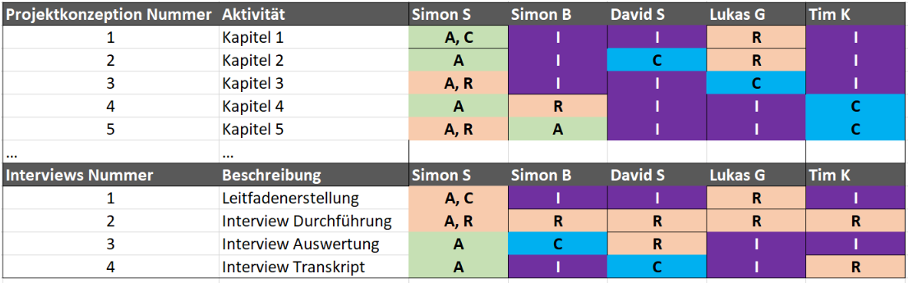
\includegraphics[width=0.9\linewidth]{graphics/raci.png}
    \caption[Die \ac{RACI}-Matrix des Projekts.]{Die \ac{RACI}-Matrix des Projekts.}\label{abb:raci}
\end{figure}
\section{Regelmäßiger Austausch}
Unabhängig davon, ob es sich um neue Entwicklungen, strategische Überlegungen, operative Angelegenheiten oder allgemeine Probleme handelt,
ist es unerlässlich, diese Themen zu diskutieren. Dafür können entweder direkt die Verantwortlichen angesprochen werden, wenn diese
existieren oder aber es wird in Regelmeetings über diese Punkte gesprochen. Jedoch führen ineffektive Regelmeetings zu verspäteten Entscheidungen,
verschwendeten Ressourcen, verpassten Möglichkeiten und jeder Menge verlorener Zeit. 
Eine Strategie und Grundsätze für Regelmeetings in einem Projekt zu etablieren und eine gewisse Qualität zu haben,
scheint daher grundsätzlich vorteilhaft zu sein. Michael C. Mankins hat in seinem Artikel im „Harvard Business Review“-Journal „Stop Wasting Valuable Time” sieben Regeln
aufgestellt, diese möglichst effektiv zu gestalten:
\begin{itemize}
    \item \textbf{Strategie und Operationen getrennt behandeln:} Strategische Themen benötigen mehr Zeit und sollten daher in separaten Meetings behandelt werden.
    \item \textbf{Fokus auf Entscheidungen, nicht Diskussionen:} Qualität und Geschwindigkeit der Entscheidungsfindung verbessern, indem beispielsweise Dokumente im Voraus verschickt werden. Dies spart jedem Teilnehmer viel Zeit und auch die Gesamtlänge des Meetings wird verkürzt.
    \item \textbf{Den wirklichen Wert jedes Tagesordnungspunktes messen:} Priorisieren der Tagesordnungspunkte nach ihrer Auswirkung auf den weiteren Verlauf des Projektes. Wichtige Punkte zuerst behandeln.
    \item \textbf{Themen schnell von der Tagesordnung abhandeln:} Klare Zeitpläne festlegen, wann und wie Teilnehmer jedes Thema entscheiden, damit nicht zu viel Zeit auf einem Thema benötigt wird.
    \item \textbf{Entscheidungen verbindlich machen:} Explizit vereinbaren, was in der Besprechung entschieden wurde. Entweder direkt während des Meetings festhalten oder eine Kommunikation im Nachgang senden.
\end{itemize}
Nachdem ein paar Grundsätze festgelegt werden, geht es an die Feinplanung der 
Regelmeetings. Im 5. Semester ist ein wöchentliches Meeting jeden Donnerstag um 16:30Uhr vorgesehen.
Der Zeitumfang beträgt dabei immer maximal eine Stunde. Wenn an diesem Tag Vorlesungen sind, wird werden die Treffen in Präsenz
im Anschluss an die Vorlesung durchgeführt, in anderen Fällen finden diese per Videokonferenz statt. Zusätzlich zu diesem festgelegten Termin wird in der Vorlesungszeit
des Kurses „Projektkonzeption“ über operative Tätigkeiten im Detail gesprochen und sich mit dem verantwortlichen Teammitgliedern abgestimmt,
um die Entstehung von Dupletten oder unbehandelten Punkten am Ende des Projekts zu vermeiden.

\chapter{Technische Realisierung}
Gegenstand der Arbeitspaketeplanung ist die Struktur von Projekten hinsichtlich ihrer Komplexität.
\footcite[Vgl.][128]{kusterHandbuchProjektmanagementAgil2022}
Dies geschieht durch die Unterteilung des Projektes in kleinere Einheiten sowie durch die Erstellung eines Projektstrukturplans.
Oftmals wird dieser einschließlich seiner Meilensteine auf Arbeitspaketebene aufgeteilt und somit für Projektmitarbeiter editierbar gemacht.
\footcite[Vgl.][121]{panagosToolsUndMassnahmen2019}
Dies ist vergleichbar mit einer umgekehrten Baumstruktur, bei welcher im oberen Bereich der jeweilige Meilenstein dargestellt ist und die Blätter die
zugehörigen Arbeitspakete repräsentieren.
\footcite[Vgl.][29]{kusay-merkleAgilesProjektmanagementIm2018}
Im unteren Bereich sind schlussendlich die unteilbaren Arbeitspakete zu finden. In der Theorie können diese jedoch auf einer beliebigen Ebene liegen.
\footcite[Vgl.][73]{gadatschGrundkursITProjektcontrollingGrundlagen2008}
Das Finden von Arbeitspaketen findet hierbei ausgehend von der unteren Ebene statt.
Diese eignet sich insbesondere für Projektvorhaben, welchen eine geringere Erfahrung mit dem zu behandelnden Themengebiet zugrunde liegt.
Hierbei werden alle Tätigkeiten als Team zusammengeführt und anschließend Meilensteine mit den darunterliegenden Arbeitspaketen
definiert (siehe Abb. \ref{abb:psp}).
\footcite[Vgl.][133]{kusterHandbuchProjektmanagementAgil2022}
\begin{figure}[H]
    \centering
    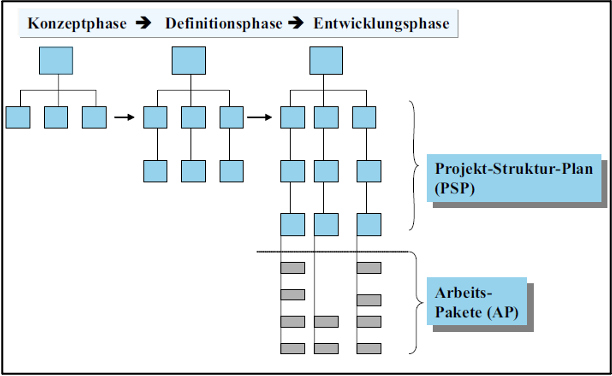
\includegraphics[width=0.47\linewidth]{graphics/psp.png}
    \caption{Zuordnung von Arbeitspaketen innerhalb der Projektstrukturplanung.}\label{abb:psp}
\end{figure}
\section{Arbeitspaketebeschreibung und Aufwandsschätzung}
Bestandteile bei der Defintion von Arbeitspaketen sind die Leistungsbeschreibung, die jeweils verantwortliche Person
sowie die zugeordneten Ressourcen.
\footcite[Vgl.][73]{gadatschGrundkursITProjektcontrollingGrundlagen2008}
Zusätzlich können untergeordnete Aufgabenpakete mit entsprechenden Zeitangaben erstellt werden.
\footcite[Vgl.][74]{gadatschGrundkursITProjektcontrollingGrundlagen2008}
Als Ergebnis muss denoch schlussendlich ein minimal funktionsfähiges Produkt (in der Literatur: „\ac{MVP}“)
vorliegen, welches im Sinne des Wasserfall-Modells in die nächste Phase übernommen werden kann.
\footcite[Vgl.][52]{panagosToolsUndMassnahmen2019}
Als weitere Anforderung an die Arbeitspakete soll beim vorliegenden Projekt dafür gesorgt sein, dass die Ausführung
von einer einzelnen Person in einem angemessenen zeitlichen Rahmen bewältigt werden kann.
In Projekten, welche unter wirtschaftlichen Rahmenbedingungen stattfinden, werden für die Schätzung des Zeitbedarfs
der einzelnen Projektaktivitäten häufig \ac{PM} benutzt, bei welchen allerdings Vollzeitmitarbeiter als Grundlage
angesehen werden.
\footcite[Vgl.][74]{gadatschGrundkursITProjektcontrollingGrundlagen2008}
Da dieser Umstand bei einem Hochschulprojekt nicht gegeben ist, wird daher mit keiner konkret geschätzten Zeit
gearbeitet. Es wird hier nach interner Absprache zwischen dem Projektteam lediglich eine Abgabefrist für
Arbeitspakete gesetzt, welche für alle am Projekt beteiligten Personen einzuhalten ist. Weitere Informationen
hierzu sind in \textit{Kapitel 6} zu finden.
\section{Backlog und Akzeptanzkriterien für Arbeitspakete}
Das Backlog stellt eine Liste der gewünschten Arbeiten dar.
\footcite[Vgl.][362]{kusay-merkleAgilesProjektmanagementIm2018}
Diese noch zu erledigenden Aufgaben können dort bis zur abschließenden Nutzung gesammelt und aufbereitet werden.
\footcite[Vgl.][362]{kusay-merkleAgilesProjektmanagementIm2018}
Ferner werden die Arbeitspakete hierbei den großen Meilensteinen (in der Literatur: „Epics“) zugeordnet.
Als Werkzeug für diese Arbeitspakete- und Zeitplanung kommt das Programm „Jira Software“ zum Einsatz.
Es ist für kleine Projekte kostenlos nutzbar und enthält Funktionen für die Nachvollziehbarkeit von Aufgaben
und Fehlern sowie für die Verwaltung von Projekten.
\footcite[Vgl.][3]{ortuMeasuringUnderstandingEffectiveness2015}
Als vorteilhaft bei der Nutzung von Jira erweist sich der grundflexible Charakter der Software, welcher
es dem Projektteam unter anderem ermöglicht, Teilinkremente mit hoher Produktivität auszuliefern, das Backlog zu verwalten
sowie den Fortschritt des Projekts visuell darzustellen.
\footcite[Vgl.][3]{ortuMeasuringUnderstandingEffectiveness2015}
Die aktuellen Meilensteine im Backlog sind folgende:
\begin{enumerate}
    \item Ausarbeitung der Projektkonzeption
    \item Präsentation am Anfang des sechsten Semesters
    \item Interviews mit Leitfaden
    \item Wissenschaftliche Ausarbeitung im sechsten Semester
    \item Prototyp im sechsten Semester
    \item Ergebnispräsentation am Ende des sechsten Semesters
\end{enumerate}
Im Backlog werden schließlich für die einzelnen Arbeitspakete der Meilensteine Kriterien erstellt, anhand derer
erkenntlich wird, ob das jeweilige Objekt den Anforderungen entsprechend umgesetzt worden ist.
\footcite[Vgl.][46]{kusay-merkleAgilesProjektmanagementIm2018}
Vor der Fertigstellung eines Arbeitspakets müssen alle vorher definierten Akzeptanzkriterien erfüllt sein.
\footcite[Vgl.][154]{kusterHandbuchProjektmanagementAgil2022}
\chapter{Schnittstellen und Zusammenarbeit mit anderen Projekten}
In Unternehmen werden Schnittstellen zwischen verschiedenen Projekten durch den Einsatz eines Projektportfolio-Managements überwacht und dirigiert.
\footcite[Vgl.][S. 356 f.]{bilginHandlingProjectDependencies2017}
Die Einflüsse der anderen Projekte werden offensichtlich, wenn die Abhängigkeiten, welche durch die Aufgabengebiete definiert sind,
dargestellt werden. Diese Einflüsse können, wie im Kapitel Risiko erläutert, überaus Einfluss auf die Qualität und die Zeitplanung des Projektes haben.
Um diesen Einfluss darstellen zu können, wird die Kontextebene des C4-Modells verwendet, um einen Überblick über die Schnittstellen zu erhalten.
\begin{figure}[H]
    \centering
    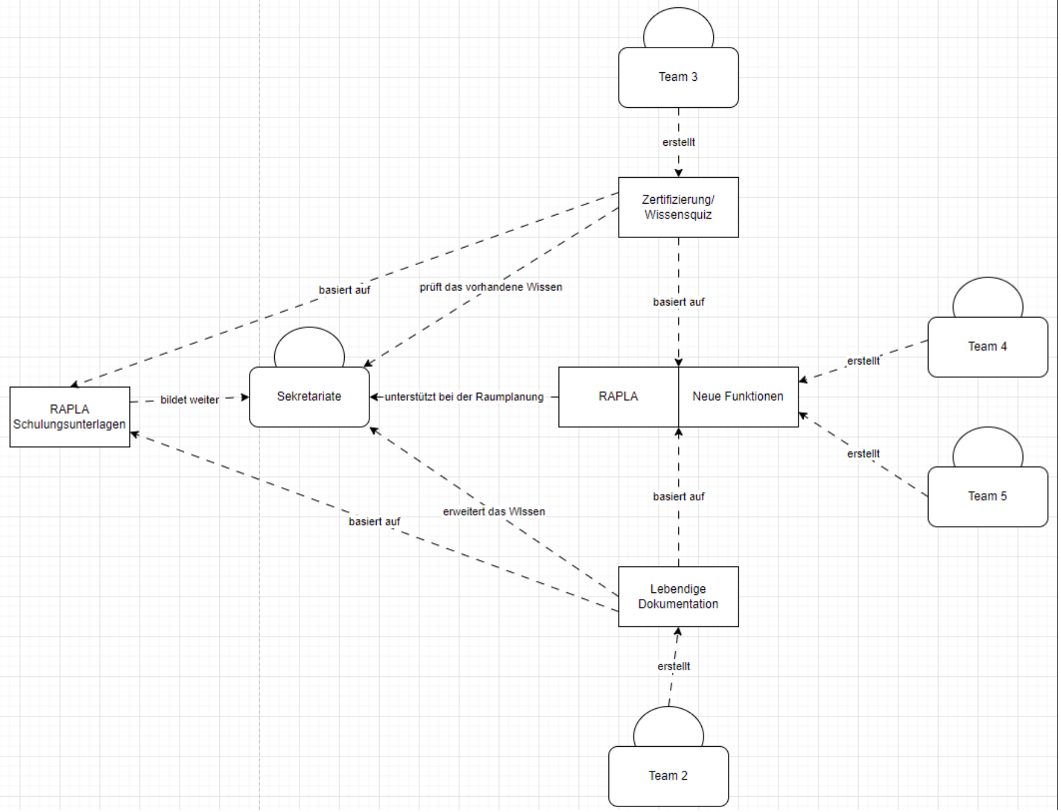
\includegraphics[width=1\linewidth]{graphics/rapla_model.png}
    \caption{Schnittstellen im vorliegenden Projekt.}\label{abb:zeitplanung}
\end{figure}
Wie an diesem Modell sichtbar, gibt es für dieses Projekt (Team drei) 
hauptsächlich eine direkte Abhängigkeit zu den Teams vier und fünf, da die
Zertifizierung bestenfalls neue Funktionen von \ac{RAPLA} berücksichtigt und prüft. Allerdings
gibt es auch eine indirekte Schnittstelle zu Team zwei, da diese ihre lebendige Dokumentation
auf den gleichen Quellen (\ac{RAPLA} und \ac{RAPLA} Schulungsunterlagen) aufbaut. Durch klare Absprache
können Mehrarbeit und Dopplungen vermieden werden.

Aufbauend auf diesen Schnittstellen wird für die Zukunft folgende Zusammenarbeits-Maxime definiert: 
Die Entwicklung der Teams vier und fünf werden verfolgt und es werden bereits vor deren Fertigstellung Platzhalter
in der Zertifizierung geschaffen, um die Entwicklungen direkt nach ihrer Fertigstellung gegebenenfalls in die
Zertifizierung aufnehmen zu können (soweit sie auch von den Schulungsunterlagen aufgenommen werden).
Während sich die Interaktion mit den Teams Teams vier und fünf eher auf die zweite Hälfte des Projektes
beziehen wird, besteht das Absprache-Potenzial mit Team zwei von Beginn an. Daher werden regelmäßige Absprachen
sowie ein Austausch von Informationen geplant. Zusätzlich werden außerplanmäßige Treffen bei der Koordination
von bestimmten Arbeitspaketen oder zu besonderen Anlässen wie Rücksprachen mit den Stakeholdern stattfinden.
\chapter{Zeitplanung}
Die Zeitplanung spielt im Kontext des Hochschulprojektes eine bedeutende Rolle,
da das Projekt zeitlich eng begrenzt und auf zwei verschiedene Semester aufgeteilt ist.
Es ergibt sich die Notwendigkeit einer detaillierten Planung, um alle Anforderungen
termingerecht erfüllen zu können und Abhängigkeiten zwischen mehreren Teammitgliedern
konfliktfrei zu lösen. Weiterhin müssen separate Planungen für die jeweiligen Semester
durchgeführt werden, da diese zwar abhängig voneinander sind, die Informationen für die
Planung des höheren Semesters allerdings noch nicht vorhanden sein müssen.

Die Planung dazu basiert - wie in vorherigen Kapiteln beschrieben - allgemein auf
festen Abgabeterminen zu bereits festgelegten Meetings. 
Begonnen wurde mit der groben Definition von Epics
und Arbeitspakten in Jira, auf deren Basis dann eine vorläufige Planung für beide Semester
erstellt wurde. Diese konnte schrittweise in ihrem Detailgrad ausgebaut werden.

Zur Visualisierung wurde die Zeitleiste in Jira verwendet, die einem Gantt-Diagramm ähnelt.
Das Gantt-Diagramm bietet sich bei der Zeitplanung hierbei besonders an, da es eine
übersichtliche Möglichkeit bietet, Verknüpfungen mit vorangehenden Vorgängen,
Dokumentation der Vorgangsverantwortlichen sowie Kapazitätsdarstellungen, in einem
Diagramm zu veranschaulichen.
\footcite[Vgl.][123]{osterhageAnhangProjektmanagement2016}
Dadurch, dass über die Zeitachse Aktivitäten in Form von Balken mit festen Anfangs-
und Endtermin dargestellt werden, können Abhängigkeiten zwischen Aufgaben und
Arbeitspaketen hergestellt sowie kritische Stellen in der Planung sichtbar gemacht
werden.
\footcite[Vgl.][117]{hobelGABLERBUSINESSWISSENAZ2006}
Zudem erklärt sich die populäre Nutzung von Gantt-Charts auch dadurch, dass
sie sowohl den Projektteilnehmern eine übersichtliche Visualisierung des Projektfortschritts
ermöglichen als auch in der finalen Präsentation der Ergebnisse vor dem Management genutzt
werden können.
\footcite[Vgl.][435]{wilsonGanttChartsCentenary2003}
\begin{figure}[H]
    \centering
    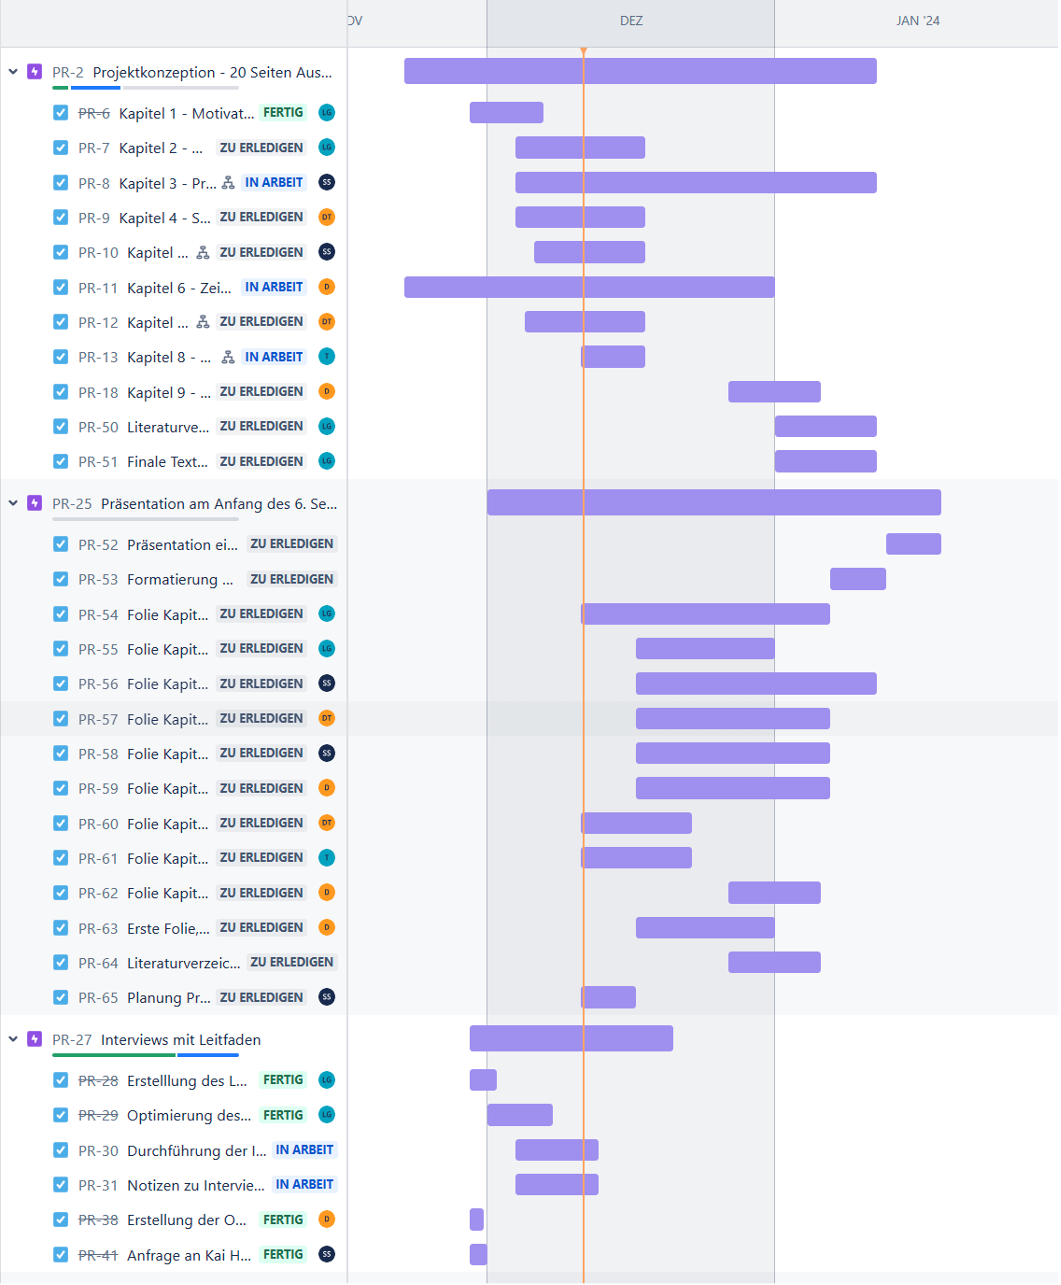
\includegraphics[width=0.9\linewidth]{graphics/zeitplanung.png}
    \caption{Übersicht über die Zeitplanung in JIRA.}\label{abb:zeitplanung}
\end{figure}
Es wird sichtbar, dass die Kapitel nach einer logischen Reihenfolge eingeteilt worden sind.
Allgemeine Planungsthemen wie Projektplanung oder
Zeitplanung sind auf einen größeren Zeitraum zugeschnitten, konkrete Kapitelthemen wie die
Einleitung oder auch die Anforderungen dagegen für kurze und spezifische Zeitperioden vorgesehen
sowie in einer für den Ablauf effizienten, sequenziellen Reihenfolge angeordnet. Hieraus ergibt
sich, dass das sechste Semester überwiegend für die Umsetzung genutzt werden kann und jegliche
Planung bereits zu großen Teilen finalisiert ist.

Bezüglich der Umsetzungsplanung lässt sich feststellen, dass die Umsetzung der Schulungsunterlage
einige Abhängigkeiten mit sich bringt. So erfordert sie enge Absprachen mit dem zweiten
Schulungs-Team, um keine Dopplungen zu erhalten. Diese Planung kann sich jedoch aufgrund
des neuen Vorlesungsplans im sechsten Semester noch ändern. 


\chapter{Risikoregister}


\chapter{Skizze der Lösungsarchitektur}
\section{Planung und Vorbereitung der Interviews}
Im Rahmen des Projekts werden diverse Interviews durchgeführt, welche ein Schlüsselelement für die Anforderungsanalyse des Projektes bilden.
Diese Methode ermöglicht umfassende Einblicke in die Nutzererfahrungen und Erwartungen an das Planungstool \ac{RAPLA}.
\footcite[Vgl.][567]{baurHandbuchMethodenEmpirischen2014}
Die zeitige Planung für dieses Semester ermöglicht es, frühzeitig wertvolle Erkenntnisse für die Projektentwicklung zu gewinnen und
strategisch in die nächste Phase des Projekts einzusteigen.
\footcite[Vgl.][568]{baurHandbuchMethodenEmpirischen2014}

\section{Entwicklung und Durchführung der Interviews}
Die Entwicklung und Durchführung der Interviews basiert auf einem wohlüberlegten und
strukturierten Ansatz, der die Tiefe und Breite der zu erforschenden Themen vollständig umfasst.
Unser umfangreicher Interviewleitfaden ist sorgfältig ausgearbeitet und orientiert
sich an einem klaren Schema (siehe Abb. \ref{abb:leitfaden}).
\begin{figure}[H]
    \centering
    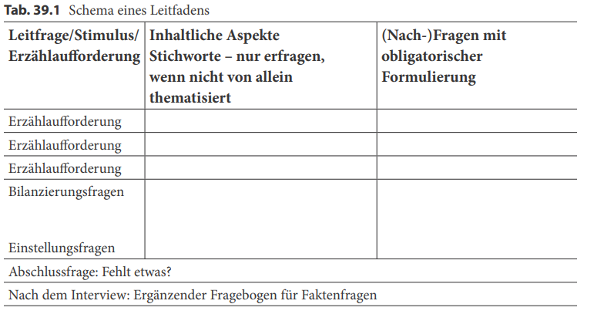
\includegraphics[width=0.9\linewidth]{graphics/leitfaden.png}
    \caption[Schema eines Leitfadens.]{Schema eines Leitfadens.\protect\footnotemark}\label{abb:leitfaden}
\end{figure}
\footnotetext{Enthalten in: \cite{baurHandbuchMethodenEmpirischen2014}, S. 568.}

Jede
Interviewphase ist mit spezifischen Zielen und Fragen verbunden, die darauf abzielen, ein
umfassendes Verständnis von den Erfahrungen der Sekretariatsmitarbeitenden mit digitalen
Werkzeugen sowie ihren Erwartungen an das Planungstool \ac{RAPLA} zu erhalten.

Die Leitfragen dienen als Orientierung für die Befragten, um die Diskussion zu initiieren und sicherzustellen,
dass alle relevanten Themenbereiche abgedeckt sind. Durch die offene Gestaltung wird den Befragten Raum für ihre
persönlichen Berichte und Erfahrungen gegeben. Diese Fragen sind durch inhaltliche Aspekte ergänzt, die als Stichworte dienen und bei
Bedarf abgefragt werden, um sicherzustellen, dass keine wichtigen Informationen ausbleiben.
Diese Stichworte werden nur erfragt, wenn die Teilnehmenden sie nicht von sich aus thematisieren, um die
Natürlichkeit des Gesprächsflusses zu bewahren.
Nachdem die Befragten ihre anfänglichen Gedanken und Erfahrungen geteilt haben, werden Erzählaufforderungen eingeführt,
um tiefere Einblicke und detailliertere Beschreibungen zu erhalten. Diese Aufforderungen helfen, die Erzählung zu
strukturieren und ermöglichen es den Teilnehmenden, ihre Gedanken und Gefühle in Bezug auf das Planungstool RAPLA
detaillierter auszuführen. 

Um ein ausgewogenes Verständnis zu erlangen, werden Bilanzierungsfragen gestellt, die es den Interviewten
ermöglichen, über ihre Erfahrungen zu reflektieren und sie in einen größeren Kontext einzuordnen. Diese Fragen
zielen darauf ab, die Vor- und Nachteile ihrer Erfahrungen mit RAPLA zu bewerten und eine Einschätzung der
Benutzerfreundlichkeit und Funktionalität des Tools vorzunehmen. 
Einstellungsfragen werden genutzt, um die subjektiven Meinungen und Einstellungen der Befragten
zu erfassen. Diese sind entscheidend, um zu verstehen, wie das Tool von den Nutzern wahrgenommen wird
und welche emotionalen und kognitiven Reaktionen es hervorruft. 

Zum Abschluss des Interviews wird die Frage „Für den Fall, dass Ihnen noch ein Aspekt gefehlt hat, welcher wäre dies?“ gestellt,
um es den Teilnehmenden zu ermöglichen,
zusätzliche Gedanken oder Themen einzubringen, die im Laufe des Interviews nicht angesprochen wurden. Dies
dient dazu, sicherzustellen, dass alle relevanten Informationen erfasst werden. 
Durch die Anwendung dieses strukturieren Leitfadens werden konsistente, vergleichbare und aussagekräftige Daten gesammelt.
\footcite[Vgl.][568]{baurHandbuchMethodenEmpirischen2014}
Diese Daten werden letztlich einer sorgfältigen Analyse unterzogen, um eine bestmögliche Anpassung an die Bedürfnisse und Erwartungen
der Nutzer zu gewährleisten.

\section{Integration des Wissensquiz und der Zertifizierung in Moodle}
Die Integration von Wissensbefragung und Zertifizierung in Moodle sind ein kritischer Schritt, um eine umfassende,
zugängliche und nutzerorientierte Bildungserfahrung zu schaffen. Im Zuge der Implementierung wurde sich
für das zweite Arbeitspaket entschieden, welches die Entwicklung und Gestaltung eines Wissensquiz umfasst, welches direkt in
Moodle abgebildet sein wird. Zusätzlich ist eine Zertifizierung zu entwerfen, die den Abschluss des Kurses bestätigt.

Bei der Erstellung des Quiz wird großer Wert darauf gelegt, dass dieses nicht nur informativ, sondern auch
interaktiv und spannend gestaltet wird. Es soll die Nutzer nicht nur testen, sondern auch
Anreize und Motivation zum Lernen bieten. Ferner wird in Betracht gezogen, Elemente der Gamifikation einzuführen.

\section{Gestaltung von Schulungsaufgaben}
Die Schulungsaufgaben werden so gestaltet, dass sie die direkte Anwendung von \ac{RAPLA} in realen Szenarien
widerspiegeln. Hierbei soll zunächst eine Einführung in das Thema mit einer entsprechenden Bearbeitung und Integration
des Nutzers erfolgen. Dadurch soll nicht nur das theoretische Verständnis gefördert werden, sondern es sollen auch praktische
Fertigkeiten geübt und verbessert werden. Darüber hinaus können Fallstudien und realitätsnahe Anwendungsszenarien einbezogen werden,
um die Relevanz und Anwendbarkeit des erlenten Wissens zu stärken.
Die Fragen sollen sowohl thereotische als auch praxisbezogene Übungen beinhalten.
Es wird eine Mischung aus verschiedenen Fragetypen angeboten, um Eintönigkeit zu vermeiden.
\footcite[Vgl.][141]{schweighoferDevelopmentQuizImplementation2019}

Insgesamt zielt die Integration der \ac{RAPLA}-Schulungsaufgaben darauf ab, eine benutzerfreundliche Ugebung zu kreieren,
welche die Nutzer motiviert und schlussendlich dazu befähigt, \ac{RAPLA} effektiv und effizient in ihrem Arbeitsalltag einzusetzen.
\footcite[Vgl.][1]{agambaExploringFacultyIntegration2012}

\section{Bedeutung von Testläufen in der Entwicklung}
Für die Entwicklung von Wissensbefragung und Zertfizierung lassen sich folgende Aspekte in Bezug auf Testläufe festhalten:
\begin{enumerate}
    \item \textbf{Frühe Fehlererkennung und Qualitätsverbesserung:} Die Durchführung von Testläufen während der Entwicklung des Moodle-Quiz ist entscheidend, um frühzeitig Fehler zu erkennen und zu beheben. Diese Vorgehensweise trägt maßgeblich zur Qualitätssteigerung des Endprodukts bei und stellt sicher, dass das Quiz den Lernbedürfnissen der Zielgruppe entspricht.
    \item \textbf{Integration von Probanden in die Konzept- und Entwicklungsphase:} Die Einbeziehung von Testern bereits in der Konzeptphase ermöglicht die Identifikation von Anforderungsdefekten vor ihrer Implementierung. Dies hilft, die Kosten für die Fehlerbehebung zu senken und beschleunigt den Entwicklungsprozess, indem ein tiefgehendes Verständnis für das Projekt entwickelt wird.
    \item \textbf{Sicherstellung der Softwarezuverlässigkeit:} Durch Pilot-Tests mit einer ausgewählten Nutzergruppe wird wertvolles Feedback gesammelt, das für die Anpassung des Quiz entscheidend ist. Diese Tests gewährleisten die Sicherheit und Zuverlässigkeit des Moodle-Quiz, indem sie sicherstellen, dass es in realen Szenarien sicher verwendet werden kann, was für die Zielgruppe von entscheidender Bedeutung ist.
\end{enumerate}
Durch diese strukturierte Einbindung von Testläufen in den Entwicklungsprozess wird sichergestellt, dass das Moodle-Quiz nicht nur fehlerfrei, sondern
auch optimal auf die Bedürfnisse und Präferenzen der Nutzer zugeschnitten ist.
\chapter{Abschließende Evaluation}
Abschließend kann festgestellt werden, dass zwar durch
einige kurzfristige Anforderungsänderungen Umplanungen notwendig
wurden, diese aber in Absprache mit dem Nachbar- sowie dem Entwicklerteam
innerhalb einer möglichst kurzen Zeit durchgeführt werden konnten, sodass
bereits Anfang des Jahres innerhalb der Projektgruppe der relevante Teil der Fragen geklärt war.

Für zukünftige Projekte sowie die Umsetzung der Zertifizierung im sechsten Semester ergeben sich einige
mögliche Implikationen. So bietet sich in folgenden Projekten die Diskussion einer agilen Arbeitsweise an,
da diese sich flexibler an Anforderungsänderungen anpassen lässt. Weiterhin sollten zeitliche Fristen enger
definiert werden, um zu verhindern, dass Fristen zwar eingehalten, aber in hohem Maße ausgereizt werden.
Darüber hinaus ist auch die Nutzung einer breiten Auswahl an verschiedenen Dokumentations-
und Kommunikationstools wie Jira, Word, WhatsApp und Discord eine mögliche Vergeudung im Sinne des Prozessmangements,
welche sich bspw. in Effizienzeinbußen und Kommunikationsproblemen äußern kann. Aus diesem Grund bietet sich auch hier
eine ausführliche Reflektion vor der Auswahl an Applikationen an. Als positiver Aspekt hat sich im Rahmen der Projektkonzeption
die problemlose Arbeitsteilung in der Gruppe erwiesen.

Die finale Evaluation der Planung lässt den Schluss zu, dass alle Schritte der Planung in der
geforderten Zeit durchgeführt wurden. Durch die detaillierte Anforderungs- und Risikoanalyse sowie
Umsetzungsplanung in Form von Arbeitspaketen ist auch für das folgende Semester eine im Zeitrahmen 
liegende Durchführbarkeit sichergestellt.

\chapter*{Anhang}
\addcontentsline{toc}{chapter}{Anhang}
\section*{Anhangverzeichnis}
\vspace{-8em}

% vor \listofanhang müssen Einrückungen angepasst werden
\abstaendeanhangverzeichnis

\listofanhang
\clearpage
\spezialkopfzeile{Anhang} % damit in der Kopfzeile das Wort "Anhang" angezeigt wird

\anhang{Projektrollen und Verantwortlichkeiten}\label{anhang:kap1}
% \anhangteil{Unterkapitel 1}\label{anhang:ukap1}
\begin{figure}[H]
  \centering
  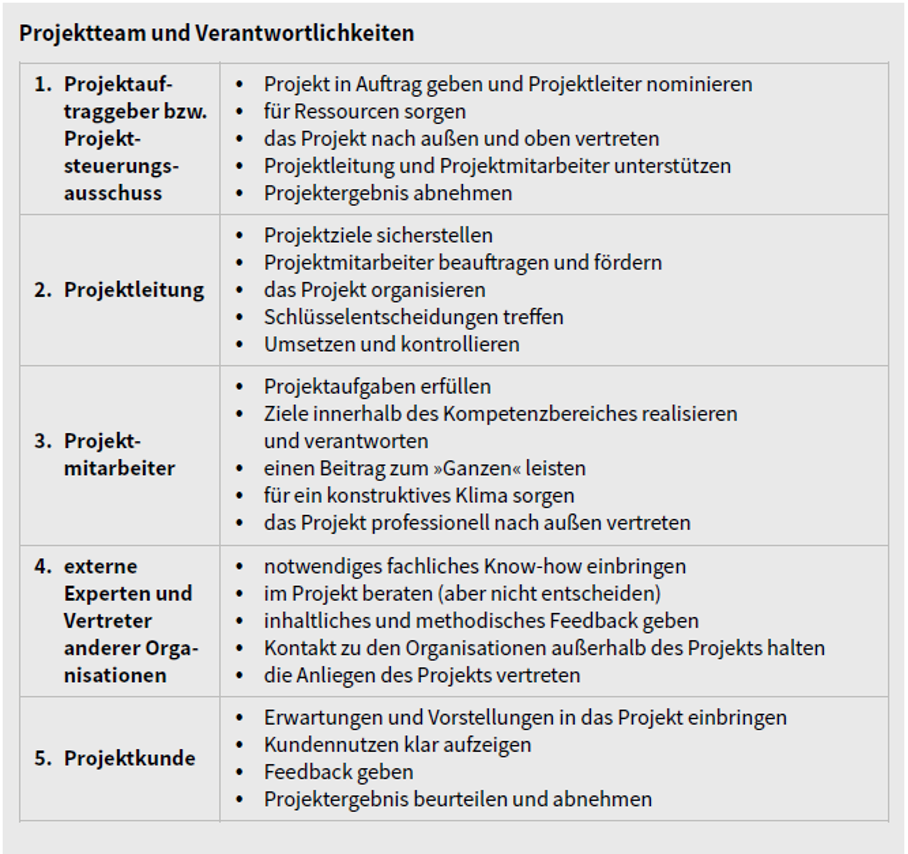
\includegraphics[width=0.8\linewidth]{graphics/pr_ve.png}
  \caption[Rollen und Verantwortlichkeiten in Projekten.]{Rollen und Verantwortlichkeiten in Projekten.\protect\footnotemark}\label{abb:pr_ve}
\end{figure}
\footnotetext{\cite[Enthalten in:][90]{stoegerWirksamesProjektmanagementMit2019}}
\anhang{Discord-Server Organisationsstruktur}\label{anhang:kap2}
\anhang{Risikomatrix}\label{anhang:kap3}


\lstset{language=TeX, % hervorzuhebende Keywords definieren
  morekeywords={anhang, anhangteil}
}

% \blinddocument
% \chapter{Beispiele für Abbildungen und Tabellen}\label{chapter:abbildungenTabellen}

Hier finden Sie Beispiele für Abbildungen, Tabellen, Formelsatz und  Source Code.

\section{Abbildungen}
In diesem Abschnitt gibt die Abbildungen~\ref{abb:Logo2cmHoch} und~\ref{abb:Logo2cmBreit}, die beide das Logo der DHBW zeigen.

\begin{figure}[htb]
\centering

\includegraphics[height=2cm]{graphics/dhbw.png}
\caption[DHBW-Logo 2cm hoch]{DHBW-Logo 2cm hoch.\footnotemark}
\label{abb:Logo2cmHoch}
\end{figure}
\footnotetext{Mit Änderungen entnommen aus: \cite{OhneAutorenOhneJahr}}

\lstset{language=TeX, % hervorzuhebende Keywords definieren
  morekeywords={footnotetext,footnotemark,footcite,caption}
}

\emph{Spezialfall:} Sofern \emph{innerhalb} der Bezeichnung einer Abbildung eine Fußnote angegeben oder eine Quelle referenziert werden soll, geschieht dies nicht per \lstinline|\footnote| oder \lstinline
|\footcite|. Vielmehr sind die Befehle \lstinline|\footnotemark| und \lstinline|\footnotetext| zu verwenden und außerdem das optionale Argument für \lstinline|\caption| anzugeben (vgl.\ Source Code).

\begin{figure}[htb]
\centering

\includegraphics[width=2cm]{graphics/dhbw.png}
\caption[DHBW-Logo 2cm breit.]{DHBW-Logo 2cm breit. (Quelle: DHBW\footnotemark)}
\label{abb:Logo2cmBreit}
\end{figure}
\footnotetext{\url{www.dhbw.de}}



\section{Tabellen}

In diesem Abschnitt gibt es zwei Beispiel-Tabellen, nämlich auf Seite~\pageref{tab:BeispielTabelleKlein} und auf Seite~\pageref{tab:BeispielTabelleGroesser}.

\begin{table}[htb]
\centering
\begin{tabular}{lcr}
links & Mitte & rechts \\
\hline
Muster & Muster & Muster \\
\end{tabular}
\caption{Kleine Beispiel-Tabelle.}
\label{tab:BeispielTabelleKlein}
\end{table}

\begin{table}[htb]
\centering
\begin{tabular}{|l|l|c|l|r||l}
    \textbf{Spalte 1} & \textbf{Spalte 2} & \textbf{Spalte 3} & \textbf{Spalte 4} & \textbf{Spalte 5} & \textbf{Spalte 6} \\
    \hline
    a        & b          & c                & d        & e        & f        \\
    Test     & Test, Test & Test, Test, Test & ~        & ~        & ~        \\
    1        & 2          & 3                & 4        & 5        & 6        \\
\end{tabular}
\caption{Größere Beispiel-Tabelle.}
\label{tab:BeispielTabelleGroesser}
\end{table}

\section{Etwas Mathematik}

Eine abgesetzte Formel:
\[
  \int_a^b x^2 \: \mathrm{d} x = \frac{1}{3} (b^3 - a^3)
\]

Es ist $a^2+b^2 = c^2$ eine Formel im Text.

\section{Source Code}

Source Code-Blöcke können auf folgende Arten eingefügt werden:

\lstset{language=Java}

Direkt im \LaTeX-Source Code:
\begin{lstlisting}
if(1 > 0) {
  System.out.println("OK"); 
} else {
  System.out.println("merkwuerdig");
}
\end{lstlisting}

oder eingefügt aus einer externen Datei.
\lstinputlisting{includes/HelloWorld.java}

% \anhang{Release Notes}
\anhangteil{Änderungen in Version 1.1}\label{anhang:ReleaseNotes11}
In Version 1.1 sind einige Rückmeldungen, die nach der Einführungsvorlesung am 6.2.2015 oder nach Veröffentlichung der Vorlage in Moodle eingegangen sind, berücksichtigt worden. Korrekturen sind mit \enquote{(Fix)} gekennzeichnet. 

\begin{itemize}
\item \verb|latex-vorlage.tex|
\begin{itemize}
\item (Fix) Abkürzungsverzeichnis wird vor Abbildungsverzeichnis platziert
\item (Fix) Abbildungs- und Tabellenverzeichnis in Inhaltsverzeichnis aufgenommen
\item (Fix) Quellenverzeichnis wird nun ohne Kapitelnummer dargestellt

\item eingebundene Dateien in Unterverzeichnissen \verb|includes| bzw.\ \verb|graphics|
\item Beispiel-Anhang (Datei \verb|anhang.tex|) mit Erklärungen wurde eingebunden 
\end{itemize}

\item \verb|_dhbw_praeambel.tex|
\begin{itemize}
\item (Fix) das Paket hyperref wird nach biblatex eingebunden, um ein Problem mit der Verlinkung der Fußnoten im PDF zu beheben
\item (Fix) Fußnoten  gemäß der Richtlinien fortlaufend nummeriert und nicht pro Kapitel
\item Einstellungen hinzugefügt, um Anhangsverzeichnis zu ermöglichen
\item bessere Kompatibilität zwischen KOMA-Script (scrreprt) und anderen Paketen mittels scrhack
\end{itemize}

\item \verb|_dhbw_biblatex-config.tex|
\begin{itemize}
\item (Fix) keine Abschnittsnummern für einzelne Verzeichnisse im Quellenverzeichnis
\end{itemize}

\item \verb|abbildungen_und_tabellen.tex|
\begin{itemize}
\item Erklärung, wie eine Fußnote/ein Zitat bei einer Abbildung zu erstellen ist
\end{itemize}

\item \verb|abkuerzungen.tex|
\begin{itemize}
\item Abkürzungsverzeichnis wird im Inhaltsverzeichnis aufgeführt
\end{itemize}

\item \verb|abstract.tex|, \verb|anhang.tex|, \verb|einleitung.tex| 
\begin{itemize}
\item Erklärungen im Text ergänzt
\end{itemize}

\item \verb|deckblatt.tex|
\begin{itemize}
\item Meta-Daten (Autor, Titel) für die generierte PDF-Datei lassen sich nun festlegen
\end{itemize}

\end{itemize}


\anhangteil{Änderungen in Version 1.2}\label{anhang:ReleaseNotes12}
Über das Forum in Moodle sind einige Rückmeldungen eingegangen -- vielen Dank an alle, die dazu beigetragen haben. In der Version 1.2 wurden folgende Änderungen vorgenommen, wobei Korrekturen wieder mit \enquote{(Fix)} gekennzeichnet sind: 

\begin{itemize}
\item \verb|latex-vorlage.tex| (Hauptdokument)
\begin{itemize}
\item (Fix) Zeile 19: Seitenzahlen zu Beginn mit römischen \emph{Groß}buchstaben nummeriert
\end{itemize}

\item \verb|_dhbw_praeambel.tex|
\begin{itemize}
\item Zeile 39/40: Unterstützung für \enquote{ebenda} 
\item Zeile 46--68: zweite Gliederungsebene für Anhänge ermöglicht
\item (Fix) Zeile 70--73: Abbildungen und Tabellen: Zähler fortlaufend, kein Rücksetzen zu Kapitelbeginn (Paket \verb|chngcntr| anstelle von Paket \verb|remreset|)
\end{itemize}

\item \verb|_dhbw_biblatex-config.tex|
\begin{itemize}
\item (Fix) bei Quellen mit Herausgeber, aber ohne Autor wird der Name des Herausgebers im Verzeichnis fett gedruckt
\item Unterstützung für \enquote{ebenda} 
\end{itemize}

\item \verb|abkuerzungen.tex|
\begin{itemize}
\item Bemerkungen zur fortgeschrittenen Nutzung des \verb|acronym|-Pakets eingefügt 
\end{itemize}

\item \verb|einleitung.tex|
\begin{itemize}
\item Abschnitt 1.3 zu Einstellungen ergänzt
\item Abschnitt 1.5 zu Fehlerbehebungen eingefügt 
\end{itemize}

\item \verb|text-mit-zitaten.tex|
\begin{itemize}
\item Abschnitt 3.1 eingefügt, Erläuterungen zum Zitieren mit \enquote{vgl.} und \enquote{ebenda}. 
\item Abschnitt 3.2: Beispiele ergänzt
\item Hinweis zu Jahreszahlen bei Online-Quellen
\end{itemize}

\item \verb|anhang.tex|
\begin{itemize}
\item Erläuterungen zur zweiten Gliederungsebene
\end{itemize}

\item \verb|literatur-datenbank.bib|
\begin{itemize}
\item weitere Beispiele für Quellen
\end{itemize}

\end{itemize}

\anhangteil{Änderungen in Version 1.3}\label{anhang:ReleaseNotes13}
Durch die ab 1/2016 geltenden Änderungen der Zitierrichtlinien des Studiengangs waren einige kleinere Anpassungen der Vorlage erforderlich, die nachfolgend beschrieben sind. Bei dieser Gelegenheit ebenfalls erfolgte Korrekturen sind wieder mit \enquote{(Fix)} gekennzeichnet:

\begin{itemize}
\item \verb|latex-vorlage.tex| (Hauptdokument)
\begin{itemize}
\item Hinweis auf Option doppelseitiger Druck entfernt
\item Schriftgröße der Kapitelüberschriften verkleinert
\item (Fix) Kopf- und Fußzeilen werden nun korrekt angezeigt für erste Seite eines Kapitels und auch  Quellenverzeichnisse
\end{itemize}

\item \verb|_dhbw_praeambel.tex|
\begin{itemize}
\item Angabe des unteren Rands für Seitenzahl, da diese nun unten rechts steht
\item Unterstützung für \enquote{ebenda} entfernt
\item (Fix) Präfixe wie \enquote{von} im Namen eines Autors werden berücksichtigt
\item Anpassung der Abstände bei Kapitelüberschriften
\item Kopf- und Fußzeile für Verzeichnisse nun in \verb|_dhbw_kopfzeilen.tex| definiert 
\end{itemize}


\item \verb|deckblatt.tex|
\begin{itemize}
\item Schriftgröße des Titels vergrößert
\item Befehl \verb|\typMeinerArbeit| eingeführt, um Typ auszuwählen
\item Festlegung des Themas (für ehrenwörtliche Erklärung) mit Befehl \verb|\themaMeinerArbeit|
\item Darstellung der Angabe des Betreuers in der Ausbildungsstätte angepasst
\item Formulierung des Sperrvermerks angepasst  
\end{itemize}

\item \verb|_dhbw_erklaerung.tex|
\begin{itemize}
\item Formulierung angepasst an geänderte Prüfungsordnung
\item Typ und Thema der Arbeit werden automatisch eingefügt
\end{itemize}

\item \verb|_dhbw_kopfzeilen.tex|
\begin{itemize}
\item Seitennummern stehen jetzt unten rechts
\item (Fix) Kopf- und Fußzeile werden nun korrekt angezeigt in Verzeichnissen und dem Anhang
\end{itemize}

\item \verb|_dhbw_biblatex-config.tex|
\begin{itemize}
\item Anpassung des Zitierstils auf die ab 1/2016 geltenden Regelungen  
\item Vorkehrungen für Eindeutigkeit (Hinzufügen abgekürzter oder nötigenfalls ausgeschriebener Vorname) bei Übereinstimmung von Name und Jahreszahl 
\end{itemize}

\item \verb|einleitung.tex|
\begin{itemize}
\item Abschnitt 1.3 zu Einstellungen grundlegend überarbeitet
\item Abschnitt 1.5.2 zur Kontrolle der Seitenränder eingefügt 
\end{itemize}

\item \verb|text-mit-zitaten.tex|
\begin{itemize}
\item Abschnitt 3.1: Hinweise zu \enquote{ebenda} entfernt
\item Abschnitt 3.2: Beispiele zur Eindeutigkeit des Zitats ergänzt
\item Abschnitt 3.3: Hinweise für E-Journals/E-Books ergänzt 
\end{itemize}

\item \verb|anhang.tex|
\begin{itemize}
\item (Fix) Befehl \verb|\spezialkopfzeile| aufgenommen, damit in Kopfzeile das Wort \enquote{Anhang} angezeigt wird 
\item diese Release Notes wurden in eine eigene Datei verschoben
\end{itemize}

\item \verb|release_notes.tex|
\begin{itemize}
\item s.o.
\end{itemize}


\item \verb|literatur-datenbank.bib|
\begin{itemize}
\item weitere Beispiele für Quellen
\end{itemize}
\end{itemize}

\anhangteil{Änderungen in Version 1.4}\label{anhang:ReleaseNotes14}
Durch nicht abwärtskompatible Änderungen beim Versionswechsel von Biblatex 3.2 zu 3.3 sind einige Änderungen notwendig geworden.\footnote{Diese basieren auf Vorschlägen von Yannik Ehlert -- vielen Dank dafür!}
Die vorliegende Version 1.4 wurde erfolgreich mit MikTeX gestestet (portable Version 2.9.6361 vom 3.6.2017, unter Verwendung von Biblatex 3.7).

\begin{itemize}
\item \verb|_dhbw_biblatex-config.tex|
\begin{itemize}
\item Anpassung der \verb|\usebibmacro|-Befehle
\end{itemize}

\item \verb|_dhbw_authoryear.bbx|
\begin{itemize}
\item  Änderung von \verb|\printdateextralabel| zu \verb|\printlabeldateextra|
\end{itemize}
\end{itemize}

\anhangteil{Änderungen in Version 1.5}\label{anhang:ReleaseNotes15}
Für den Test dieser Version auf einem Windows-System wurde wieder die portable Version von MiKTeX (2.9.6521 vom 10.11.2017) verwendet.\footnote{\url{http://miktex.org/portable}} Da in diesem Paket leider die Versionen von Biblatex (3.10) und Biber (2.7) inkompatibel sind, ist es erforderlich, die Datei \verb|biber.exe| im Verzeichnis \verb|texmfs\install\miktex\bin\| durch die aktuelle Version 2.10 vom 20.12.2017\footnote{\url{https://sourceforge.net/projects/biblatex-biber/files/biblatex-biber/current/binaries/Windows/}} zu ersetzen. Im Editor TeXworks verwendet man dann zum Übersetzen des \LaTeX-Sourcecodes Typeset/pdfLaTeX bzw.\ Typeset/Biber.

Korrekturen sind wieder mit \enquote{(Fix)} gekennzeichnet.

\begin{itemize}
\item \verb|latex-vorlage.tex| (Hauptdokument)
\begin{itemize}
\item Nach der Änderung der Zitierrichtlinien gibt es nun kein separates Verzeichnis mehr für Internet- und Intranetquellen.
\item Option \verb|notkeyword=ausblenden| bei \verb|\printbibligraphy| sorgt dafür, dass Sekundärliteratur korrekt zitiert wird.
\end{itemize}

\item \verb|_dhbw_praembel.tex|
\begin{itemize}
\item (Fix) Die Bezeichnung geschachtelter Anhänge wurde auf das in den Zitierrichtlinien geforderte Format \enquote{Anhang 2/1} angepasst (Befehl \verb|\anhangteil|).
\end{itemize}

\item \verb|einleitung.tex|
\begin{itemize}
\item Hinweis zum Ausblenden der farbigen Links im PDF hinzugefügt
\end{itemize}

\item \verb|text-mit-zitaten.tex|
\begin{itemize}
\item Abschnitt 3.4 aktualisiert nach Wegfall des separaten Verzeichnisses für Internet- und Intranetquellen
\item Abschnitt zum Zitieren von Sekundärliteratur hinzugefügt
\end{itemize}

\end{itemize}


\anhangteil{Änderungen in Version 1.6}\label{anhang:ReleaseNotes16}
Diese Version wurde auf einem Windows-System erfolgreich mit der portablen Version von MiKTeX (2.9.6621 vom 18.02.2018) getestet.\footnote{Vielen Dank an Florian Eichin für seine wertvollen Anmerkungen.}

Korrekturen sind wieder mit \enquote{(Fix)} gekennzeichnet.

\newpage

\begin{itemize}
\item \verb|latex-vorlage.tex| (Hauptdokument)
\begin{itemize}
\item (Fix) An einer Stelle gab es in Version 1.5 (Internetquellen nicht mehr separat) noch ein Überbleibsel von Version 1.4 (Internetquellen separat), dies wurde korrigiert.
\item (Fix) Im Inhaltsverzeichnis war die Verlinkung des Abbildungs- und Tabellenverzeich\-nisses nicht ganz korrekt.
\item Mit den Befehlen \verb|\literaturverzeichnis| bzw.\ \verb|\literaturUndQuellenverzeichnis| kann bequem die Erstellung der Quellenverzeichnisse gesteuert werden, abhängig davon, ob es ein Gesprächsverzeichnis gibt oder nicht.
 
\end{itemize}

\item \verb|_dhbw_praembel.tex|
\begin{itemize}
\item Einrückungen für Abbildungs-, Tabellen- und Anhangverzeichnis angepasst
\item Abkürzungen \enquote{Abb.} und \enquote{Tab.} für Abbildungen bzw.\ Tabellen
\end{itemize}

\item \verb|_dhbw_biblatex-config.tex|
\begin{itemize}
\item Befehle \verb|\literaturverzeichnis| und \verb|\literaturUndGespraechsverzeichnis| definiert
\item Befehl \verb|\footcitePrimaerSekundaer| definiert
\end{itemize}

\item \verb|_dhbw_erklaerung.tex|
\begin{itemize}
\item Eintrag als \enquote{Erklärung} (statt \enquote{Ehrenwörtliche Erklärung}) ins Inhaltsverzeichnis
\end{itemize}

\item \verb|einleitung.tex|
\begin{itemize}
\item Bezeichnung \enquote{Erklärung} statt \enquote{Ehrenwörtliche Erklärung}
\item Erläuterung von \verb|\literaturverzeichnis| und \verb|\literaturUndGespraechsverzeichnis|
\item Hinweis auf Notwendigkeit von Updates bei MikTeX Portable
\end{itemize}

\item \verb|text_mit_zitaten.tex|
\begin{itemize}
\item Erläuterungen zu Befehl \verb|\footcitePrimaerSekundaer| ergänzt
\end{itemize}

\item \verb|anhang.tex|
\begin{itemize}
\item Befehl \verb|\abstaendeanhangverzeichnis| für Anpassung Einrückung ergänzt
\end{itemize}

\item \verb|literatur-datenbank.bib|
\begin{itemize}
\item Eintrag ergänzt
\end{itemize}

\end{itemize}

\anhangteil{Änderungen in Version 1.7}\label{anhang:ReleaseNotes17}
Diese Version wurde auf einem Windows-System erfolgreich mit der portablen Version von MiKTeX (2.9.6942 vom 04.01.2019) getestet.

Korrekturen sind wieder mit \enquote{(Fix)} gekennzeichnet.

\begin{itemize}
\item \verb|_dhbw-authoryear.bbx|
\begin{itemize}
\item Da \verb|labeldate| in Biblatex nicht mehr unterstützt wird, erfolgte eine Umbenennung in 
\verb|labeldateparts|.\footnote{vgl.\ \url{https://github.com/semprag/biblatex-sp-unified/issues/23}}
\end{itemize}

\item \verb|_dhbw_biblatex-config.tex|
\begin{itemize}
\item (Fix) Es wurde das Problem behoben, dass im Literaturverzeichnis bei bestimmten Eintragstypen der Titel in Anführungszeichen steht.\footnote{Danke an Florian Eichin für seinen Hinweis.}
\end{itemize}

\end{itemize}


\anhangteil{Änderungen in Version 1.8}\label{anhang:ReleaseNotes18}
Diese Version wurde auf einem Windows-System erfolgreich mit der portablen Version von MiKTeX (2.9.6942 vom 04.01.2019) getestet.

Die Aktualisierungen in der Vorlage spiegeln zum Einen die Änderungen in den Zitierrichtlinien wieder. Zum Anderen wurden einige studentische Vorschläge aufgegriffen, um die Nutzung der Vorlage zu erleichtern.\footnote{Danke an Bjarne Koll, Tobias Schwarz und Lars Ungerathen für ihre Anregungen.} 

\begin{itemize}

\item \verb|latex_vorlage.tex| (Hauptdokument)
\begin{itemize}
\item Es wird nun davon ausgegangen, dass die zur Vorlage gehörenden Dateien in einem eigenen Verzeichnis (\verb|template|) liegen.
\item Stellenweise wurden Erläuterungen als Kommentare hinzugefügt.
\end{itemize}

\item \verb|_dhbw_biblatex-config.tex|
\begin{itemize}
\item Code, der mehrere Quellenverzeichnisse unterstützt, wurde entfernt.
\item Ein zu großer Abstand nach Zitaten von Sekundärliteratur wurde korrigiert. 
\end{itemize}

\item \verb|_dhbw_erklaerung.tex|
\begin{itemize}
\item Gemäß der Anforderung in den Zitierrichtlinien wird die Erklärung nicht ins Inhaltsverzeichnis aufgenommen und nicht mit einer Seitenzahl versehen. 
\end{itemize}

\pagebreak
\item \verb|_dhbw_praeambel.tex|
\begin{itemize}
\item Gemäß der Anforderung in den Zitierrichtlinien werden im Literaturverzeichnis alle Autor/innen eines Werks angegeben.
\end{itemize}

\item \verb|abstract.tex|
\begin{itemize}
\item Hinweis auf \LaTeX-Spickzettel hinzugefügt.
\end{itemize}

\item \verb|deckblatt.tex|
\begin{itemize}
\item Vorname, Name, Titel der Arbeit sind nur zu Beginn einzutragen und werden dann an den entsprechenden Stellen automatisch ergänzt.
\item Hervorhebung, dass Angaben zum Unternehmen sowie den Betreuer/innen zu ergänzen sind. 
\item Wortlaut des Vertraulichkeitsvermerks wurde an die aktuelle Fassung in der Studien- und Prüfungsordnung angepasst. 
\end{itemize}

\item \verb|einleitung.tex|
\begin{itemize}
\item Ein eigenständiges Gesprächsverzeichnis als Teil des Quellenverzeichnisses ist in den Zitierrichtlinien nicht mehr vorgesehen, die entsprechenden Hinweise wurden entfernt.
\item Ein alter Hinweis auf die Darstellung von Links im Verzeichnis der Internetquellen wurde entfernt, da es ein solches eigenständiges Verzeichnis nicht mehr gibt. 
\end{itemize}

\item \verb|text_mit_zitaten.tex|
\begin{itemize}
\item Es wird nun erläutert, wie zwei Quellenangaben unmittelbar nebeneinander dargestellt werden können.
\item Erklärungen, die von mehreren Quellenverzeichnissen ausgegangen sind, wurden entfernt.
\end{itemize}

\item \verb|literatur-datenbank.bib|
\begin{itemize}
\item Gespräch wurde entfernt, da dieses nicht mehr im Quellenverzeichnis aufgeführt werden soll.
\end{itemize}

\end{itemize}

\anhangteil{Änderungen in Version 1.9}\label{anhang:ReleaseNotes19}
Durch die Aktualisierung der Zitierrichtlinien 07/2023 haben sich nur kleinere Änderungen ergeben, die diese Version der \LaTeX-Vorlage umsetzt.

\emph{Hinweis:} Die in den Zitierrichtlinien vorgenommenen Änderungen bzgl.\ der Darstellung der Einträge im Literaturverzeichnis betreffen nicht die \LaTeX-Vorlage (vgl.\ S.\ 9), weshalb in diesem Punkt keine Anpassung erfolgte.

\begin{itemize}

\item \verb|_dhbw_erklaerung.tex|
\begin{itemize}
\item In der ehrenwörtlichen Erklärung wird der Typ der Arbeit nicht mehr ausgegeben.
\end{itemize}

\item \verb|deckblatt.tex|
\begin{itemize}
\item Auf dem Deckblatt wird \enquote{Fakultät für Wirtschaft und Gesundheit} anstelle von \enquote{Fakultät für Wirtschaft} aufgeführt.
\end{itemize}


\end{itemize}

%%% Ende des eigentlichen Inhalts %%%


%%% Quellenverzeichnisse (keine Anpassung nötig) %%%
\clearpage
\literaturverzeichnis
%%% Ende Quellenverzeichnisse %%%


%%% Erklärung (keine Anpassungen nötig) %%%
% steht ganz am Ende des Dokuments
\cleardoublepage
% \clearpage

\thispagestyle{empty}

{\LARGE\textsf{\textbf{Erklärung}}\bigskip}

% \typMeinerArbeit und \themaMeinerArbeit werden in deckblatt.tex definiert
Ich versichere hiermit, dass ich die vorliegende Arbeit mit dem Thema: \emph{\themaMeinerArbeit} selbstständig verfasst und keine anderen als die angegebenen Quellen und Hilfsmittel benutzt habe.
Ich versichere zudem, dass die eingereichte elektronische Fassung mit der gedruckten Fassung übereinstimmt.

\vspace{3cm}

\begin{center}
\begin{tabular}{ccc}
(Ort, Datum) & \hspace{0.3\linewidth} & (Unterschrift)
\end{tabular}
\end{center}
\end{document}